\documentclass[10pt,a4paper]{article}
\usepackage[margin=2cm]{geometry}
\usepackage{amsmath,amssymb,booktabs,graphicx,float,caption,tikz,xcolor,needspace,longtable}
\usepackage[hidelinks]{hyperref}
\usetikzlibrary{arrows.meta,positioning}
\graphicspath{{../../results/figures/}}
\captionsetup{font=small,labelfont=bf}
\setlength{\parskip}{5pt}\setlength{\parindent}{0pt}
\newcommand{\tablein}[1]{\input{tables/#1.tex}}
% every picture or table is tagged with where its pictures came from
\newcommand{\SYN}{\textcolor{orange!85!black}{\textbf{[SYNTHETIC]}}}
\newcommand{\REAL}{\textcolor{teal!80!black}{\textbf{[REAL]}}}
\newcommand{\BOTH}{\textcolor{violet}{\textbf{[REAL vs SYNTHETIC]}}}
\tikzset{box/.style={draw,rounded corners,fill=blue!6,minimum height=7mm,align=center,font=\small},arr/.style={-{Stealth},thick}}

\title{Seeing Through Haze, Water, Glass and Plastic\\\large Can classical image processing restore the picture? A simple walk-through}
\author{Shaik Areesh, Noel Alex Jacob, Sri Harshit K\\ Digital Image Processing (CS7.404), IIIT Hyderabad}
\date{4 November 2026 (presentation 12 November)}

\begin{document}
\maketitle
\begin{center}\begin{tabular}{lr}\toprule
\textbf{Team Members} & Student ID\\\midrule
\textbf{Shaik Areesh} & 2026909008\\
\textbf{Noel Alex Jacob} & 2025201085\\
\textbf{Sri Harshit K} & 2024102022\\\bottomrule
\end{tabular}\end{center}

\begin{abstract}\noindent
We take pictures that were spoiled by haze, murky water, rain on glass or cloudy plastic, and try to repair them using classical image-processing tools only (no machine learning). The well-known Dark Channel Prior (DCP) is our baseline. Because real spoiled pictures with a known ``clean'' answer are rare, we also \emph{make} spoiled pictures ourselves (\SYN). A large part of this report asks: \emph{can the made-up pictures be trusted to predict what happens on real ones?} The short answer: partly. They agree well for glass; for haze the full ranking of methods agrees only moderately (rank correlation +0.30 with our calibrated haze and +0.57 with the original haze on 90 scenes, and only +0.09 on outdoor scenes), though the verdict about DCP is the same.
\end{abstract}

\paragraph{How to read the tags.} Every figure and table says where its pictures came from: \SYN\ pictures we made from clean photos (the true answer is known exactly), \REAL\ photographs that were really spoiled and have a clean twin, or \BOTH\ a comparison between the two.

\tableofcontents

%--------------------------------------------------------------------
\section{The question, in plain words}
A hazy photo looks grey and flat. A photo through rain-spotted glass has blurry blobs. Underwater photos look blue-green. Can we undo this with the tools taught in a first image-processing course: stretching contrast, equalising histograms, filtering, working in the frequency domain, and so on?

We ask four things:
\begin{enumerate}
\item What does each ``spoiling medium'' actually do to light?
\item Which classical method repairs each medium best, and does anything beat DCP?
\item Does the order of steps matter (for example, sharpen then equalise, or equalise then sharpen)?
\item Can pictures we make by computer stand in for real ones?
\end{enumerate}
\paragraph{How the report builds up.} Each section uses only what the earlier ones introduced.
\begin{center}\small\begin{tabular}{p{1.2cm}p{14.3cm}}\toprule
\ref{sec:media} & \textbf{What a spoiling medium does to light}: one equation, then each medium and its frequency signature.\\
\ref{sec:data} & \textbf{The pictures we use}: made-up (synthetic) and real, and why we need both.\\
\ref{sec:methods} & \textbf{The repair methods}: every technique explained in a line, the pipelines (flow diagrams and pictures of each step), and how we score.\\
\ref{sec:synthetic} & \textbf{Results on made-up pictures}, where the true answer is known.\\
\ref{sec:real} & \textbf{Results on real pictures}, haze, raindrops and underwater.\\
\ref{sec:compare} & \textbf{Can made-up pictures stand in for real ones?} Seven tests.\\
\ref{sec:local} & \textbf{Global or local}: should a method act on the whole picture or tile by tile?\\
\ref{sec:why} & \textbf{Why it works this way}, then conclusions and limits.\\\bottomrule
\end{tabular}\end{center}


%--------------------------------------------------------------------
\section{What a spoiling medium does to light}\label{sec:media}
\subsection{One idea covers almost everything}
Light from the scene passes through the medium on its way to the camera. Two things happen:
\begin{itemize}
\item the medium \textbf{lets only a fraction $t$ of the scene light through} (so the scene looks fainter), and
\item the medium \textbf{adds light of its own}, a milky glow of brightness $A$.
\end{itemize}
Written as an equation, with $J$ the clean scene and $I$ the picture we see:
\begin{equation}
I \;=\; t\,J \;+\; A\,(1-t).
\end{equation}
If $t=1$ nothing is lost. If $t$ is near 0 we see only the glow $A$. In fog, $t$ gets smaller the farther away something is: $t=e^{-\beta d}$ with distance $d$ and fog thickness $\beta$.

\begin{figure}[H]\centering
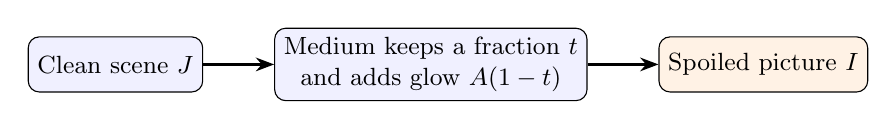
\begin{tikzpicture}[node distance=9mm]
\node[box](a){Clean scene $J$};
\node[box,right=of a](b){Medium keeps a fraction $t$\\and adds glow $A(1-t)$};
\node[box,right=of b,fill=orange!10](c){Spoiled picture $I$};
\draw[arr](a)--(b);\draw[arr](b)--(c);
\end{tikzpicture}
\caption{The one idea behind haze, water, glass film and plastic. What differs is where $t$ and $A$ come from.}\end{figure}

\subsection{The four media}
\begin{center}\small\begin{tabular}{p{2.1cm}p{6.2cm}p{7.3cm}}\toprule
Medium & What it does & Difference from plain haze\\\midrule
Haze & Fraction $t$ falls with distance; grey-white glow. & The base case.\\
Water & Same, but red light dies first, so far things turn blue-green. & Each colour has its own $t$; the glow is dark blue-green, not bright.\\
Glass & A milky film, smudges, and \emph{raindrops}. Drops act like tiny lenses that replace small patches of the scene. & Raindrops are patches, not a smooth veil.\\
Plastic & Dims, tints (often yellow), \emph{blurs} slightly, and adds a veil. & The blur is new; it is the same everywhere (not distance-dependent).\\\bottomrule
\end{tabular}\end{center}
\paragraph{The same four media in the literature's terms.}
\begin{center}\small\begin{tabular}{p{1.4cm}p{4.6cm}p{4.4cm}p{4.8cm}}\toprule
Medium & Typical cause & Visual result & Standard term\\\midrule
Air & smoke, dust, fog, humidity & grey or blue wash, distant detail lost & \textbf{atmospheric attenuation} (scattering and airlight)\\
Water & algae, sand, plankton, floating particles & green or blue tint, strong contrast loss & \textbf{turbidity} and \textbf{backscatter}\\
Plastic & polymer crystals, surface scratches & milky, cloudy or semi-opaque & \textbf{material haze} (ASTM D1003: the share of transmitted light scattered by more than 2.5 degrees)\\
Glass & smudges, dust, condensation, texture & halos around lights, washed-out contrast & \textbf{veiling glare} and \textbf{smudge flare}\\\bottomrule
\end{tabular}\end{center}
In our equations: atmospheric attenuation and backscatter are both the $tJ+A(1-t)$ of Section~\ref{sec:media}; our plastic model (blur, tint and a milky veil) stands in for material haze; our glass film and smudge stand in for veiling glare.

When two media are stacked (say, murky water seen through plastic), the equation is simply applied twice: $I_2 = t_1 t_2 J + t_2 A_1(1-t_1) + A_2(1-t_2)$.

\subsection{What this means for frequencies (a second view)}
Splitting a picture into coarse and fine detail (the Fourier transform) gives a neat summary of what each medium does:
\begin{itemize}
\item \textbf{Haze:} every level of detail is multiplied by $t$; only the average brightness gets the glow. Haze therefore \emph{fades detail evenly}.
\item \textbf{Plastic:} fades detail like haze, \emph{and} kills fine detail more than coarse detail (blur).
\item \textbf{Water:} like haze but with a different $t$ for red, green and blue.
\item \textbf{Stacks:} the effects multiply.
\end{itemize}
We checked these predictions on our made-up pictures: they hold essentially exactly (Appendix~A). The full derivations, with a literature check, are in \texttt{docs/model-equations.md}.

%--------------------------------------------------------------------
\section{The pictures we use}\label{sec:data}
We need pairs: a spoiled picture and the clean picture it came from, so we can score a repair.

\begin{center}\small\begin{tabular}{p{2.6cm}p{6.7cm}p{6.3cm}}\toprule
 & \SYN\ made by us & \REAL\ photographed\\\midrule
Haze & Clean indoor photos (NYU Depth v2, 24 rooms) with their measured depth are fogged with the equation above; 3 strengths. & O-HAZE, I-HAZE, Dense-Haze, NH-Haze (a fog machine was used and the same scene photographed with and without): 185 pairs.\\
Water & Same, with per-colour attenuation. & (a) TUB: 1,183 pairs from a water tank in which milk was added in 10 steps, camera and objects fixed, so each turbid picture has a near-clear twin (the least turbid picture of the same view). (b) UIEB: 150 ocean and reef photos with \emph{no} clean twin, so only reference-free scores.\\
Glass & Same, rain drops and film. & RainDrop dataset (58 photos of a pane with drops and the same pane clean).\\
Plastic & Same, blur and tint. & \textbf{None exists.} Own captures are planned.\\\bottomrule
\end{tabular}\end{center}

\paragraph{Why use made-up pictures at all?} Their true answer is exact, we can make as many as we like at any strength, and we can test one thing at a time. \paragraph{What is the catch?} Our equation is a model: if it is wrong, methods may look good on made-up pictures and still fail on real ones. Section~\ref{sec:compare} measures how big that catch is.

\begin{figure}[H]\centering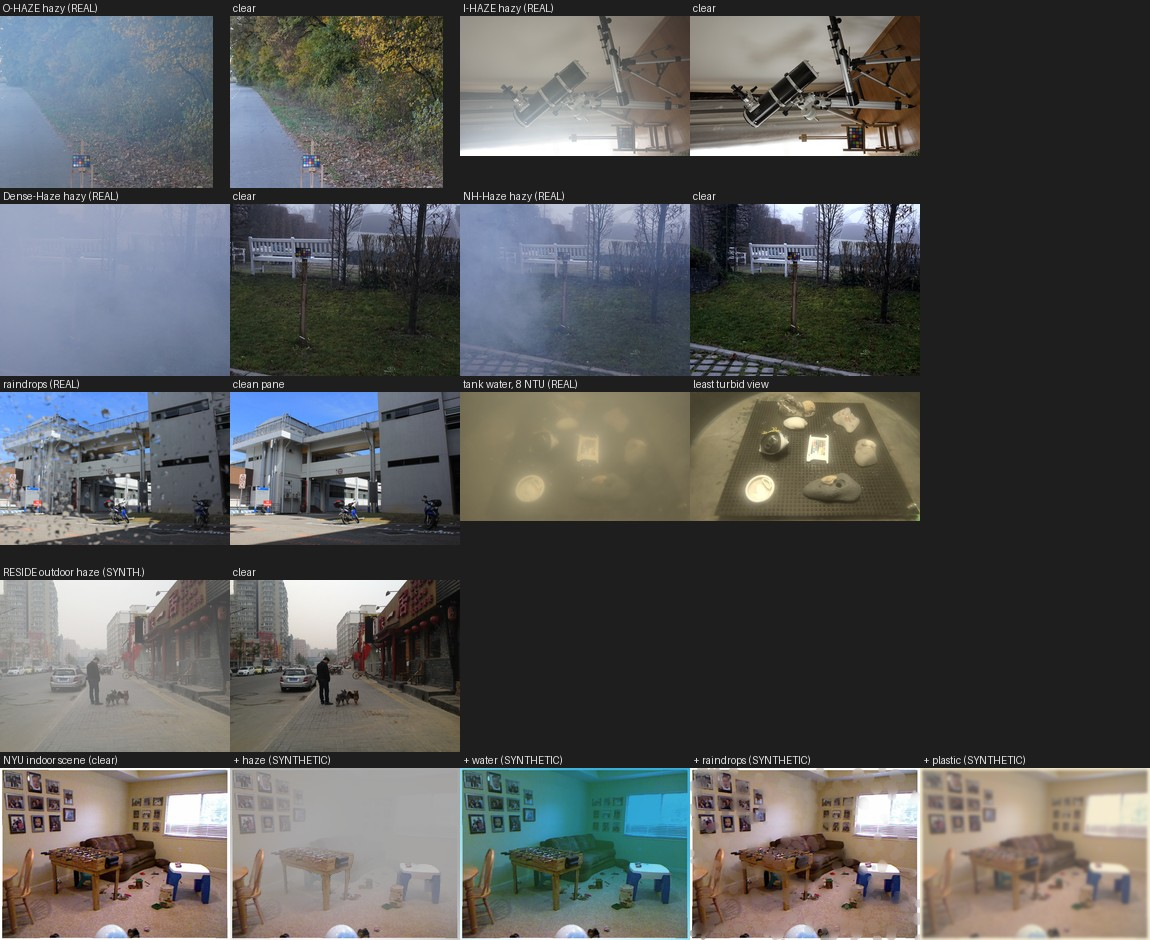
\includegraphics[width=.9\textwidth]{data_gallery.jpg}\caption{A sample from each source (spoiled picture, then its clear twin where there is one). Rows 1 to 2: real haze (O-HAZE, I-HAZE, Dense-Haze, NH-Haze). Row 3: real raindrops and real tank water. Row 4: outdoor haze made by the RESIDE authors. Row 5: one clear NYU indoor scene and the same scene degraded by each of our four models (\SYN). The UIEB ocean photos are shown in Section~\ref{sec:real}.}\end{figure}
\begin{table}[H]\centering\resizebox{\textwidth}{!}{\small\begin{tabular}{p{1.2cm}p{3.1cm}p{4.9cm}p{1.7cm}p{6.6cm}}\toprule
Medium & Cause & Data we have & Coverage & More datasets found (not downloaded)\\\midrule
Air & fog & O-HAZE, I-HAZE, Dense-Haze, NH-Haze (real fog-machine pairs, 185); RESIDE (outdoor, made) & covered & --\\
Air & smoke & NH-Haze (uneven machine fog, as a stand-in) & partly & A2I2-Haze: real smoke-machine pairs from the air and the ground, with in-place smoke measurements; behind a login and a consent notice, terms not stated\\
Air & dust, humidity & none & missing & none found\\
Water & turbidity, backscatter & TUB tank pairs (milk, near-clear reference) & covered, with a caveat (milk) & TURBID (milk, chlorophyll, blue-dye subsets with a clear reference; source not found); UFEN (talcum powder, with turbidity readings); SOTRUE (stereo, turbid; not checked)\\
Water & green or blue tint & UIEB ocean photos, no reference & partly & TURBID blue-dye subset (clear reference)\\
Water & algae, sand, plankton & none & missing & TURBID chlorophyll subset (closest to algae); UFEN talcum powder (as fine sediment)\\
Plastic & material haze, scratches & none (synthetic model only) & missing & none public; papers use ground-glass diffusers with a clear reference but release no data\\
Glass & raindrops & RainDrop pairs (58) & covered & Eigen et al. 2013 (dirt and rain on windows); ``Seeing through Unclear Glass'' (release unconfirmed)\\
Glass & smudges, dust, condensation & none (synthetic film and smudge) & missing & Flare7K++ (962 real flare photos taken through dusty and scratched lenses; non-commercial; Google Drive and Baidu)\\
Glass & halos around lights & none & missing & Flare7K++ (night-time flare)\\
Stacks & several media at once & none (synthetic only) & missing & none found\\\bottomrule
\end{tabular}}\caption{Coverage of the causes in the table above by the data we have, and what else exists. ``Covered'' means real pictures with a clean reference.}\end{table}
\begin{table}[H]\centering\resizebox{\textwidth}{!}{\scriptsize\tablein{data_matrix}}\caption{Which pictures exist and which are actually scored. ``Main comparison'' is the first method-by-method comparison (Section~\ref{sec:synthetic} and~\ref{sec:real}); the last column lists the largest other uses.}\end{table}

%--------------------------------------------------------------------
\section{The repair methods and how we score them}\label{sec:methods}
\subsection{The baseline: Dark Channel Prior (DCP)}
In most clean outdoor photos, a small patch contains at least one very dark pixel. In haze, that pixel is lifted by the glow. So the \emph{darkest value in each patch} tells us how thick the haze is there. DCP uses this to guess $A$ and $t$ and then solves the equation backwards: $J=(I-A)/t+A$.

\begin{figure}[H]\centering\resizebox{\textwidth}{!}{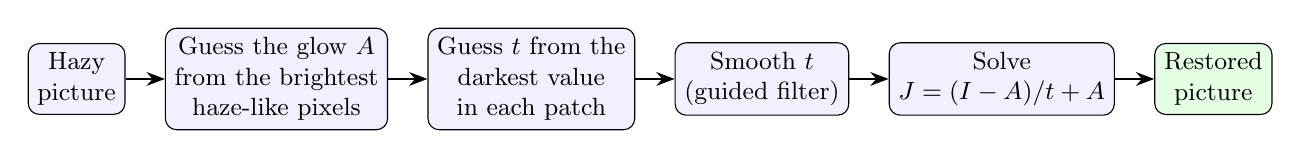
\begin{tikzpicture}[node distance=5mm]
\node[box](a){Hazy\\picture};
\node[box,right=of a](b){Guess the glow $A$\\from the brightest\\haze-like pixels};
\node[box,right=of b](c){Guess $t$ from the\\darkest value\\in each patch};
\node[box,right=of c](d){Smooth $t$\\(guided filter)};
\node[box,right=of d](e){Solve\\$J=(I-A)/t+A$};
\node[box,right=of e,fill=green!10](f){Restored\\picture};
\foreach \x/\y in {a/b,b/c,c/d,d/e,e/f}{\draw[arr](\x)--(\y);}
\end{tikzpicture}}\caption{DCP, the baseline.}\end{figure}
DCP assumes bright glow and dark pixels in clear scenes. That is a good match for haze and a poor one for water (dark blue-green glow) or plastic.

\subsection{The tools, one by one}
\label{sec:tools}
Every method below takes one picture and returns one picture. In the experiments they are called by the short names in the first column. The third column says what you \emph{see} and what the method \emph{assumes}: when the assumption is false, the method fails.

{\small\renewcommand{\arraystretch}{1.12}
\begin{longtable}{p{2.7cm}p{6.5cm}p{6.4cm}}
\toprule Name & What it does & Visible effect and assumption\\\midrule\endhead
\multicolumn{3}{l}{\textbf{Brightness and contrast} (act on the brightness values only)}\\
\texttt{stretch} & Maps the darkest 1\% of values to black and the brightest 1\% to white, linearly in between. & Fills the full range. Assumes the picture is a dimmed version of a good one.\\
\texttt{hist\_eq} & Histogram equalisation of the lightness: spreads the brightness values evenly over the range. & Strong contrast, can look harsh. Assumes an even spread of brightness is a good picture.\\
\texttt{hist\_eq\_rgb}, \texttt{eq\_hsi}, \texttt{eq\_avg\_hist} & The same, but per colour channel, on the intensity only (keeps hue), or towards the average of the three channel histograms. & Per-channel can shift colours; the others keep colours steadier.\\
\texttt{hist\_spec} & Histogram specification: reshapes the histogram into a chosen bell curve. & Natural-looking mid-tones.\\
\texttt{clahe} & Contrast-limited adaptive equalisation: equalises each tile of the picture separately (with a limit on how much it may boost) and blends. & Local contrast and detail. Can add noise or halos.\\
\texttt{gamma\_auto}, \texttt{power\_law} & A power curve $I^\gamma$; \texttt{gamma\_auto} picks $\gamma$ so the average brightness becomes 0.5. & Brightens dark pictures without clipping. Assumes the picture is just too dark.\\
\texttt{log} & $\log(1+I)$: stretches the dark values, squeezes the bright ones. & Lifts shadows.\\
\addlinespace\multicolumn{3}{l}{\textbf{Colour correction}}\\
\texttt{gray\_world} & Scales each colour so the picture's average is grey. & Removes a tint. Wrong when the scene is really one colour.\\
\texttt{white\_patch} & Scales each colour so its brightest values become white. & Removes a tint. Fooled by one coloured highlight.\\
\texttt{shades\_of\_gray} & Between the two above: estimates the light colour with a power mean. & A compromise.\\
\texttt{von\_kries} & White balance done on the eye's cone responses instead of red-green-blue. & Natural-looking neutral colours.\\
\texttt{red\_comp} & Adds red back where red is weak: $R'=R+(\bar G-\bar R)(1-R)G$. & Undoes the loss of red in sea water. Assumes red is the missing colour.\\
\addlinespace\multicolumn{3}{l}{\textbf{Haze and veil removal}}\\
\texttt{dcp}, \texttt{dcp\_guided} & Dark Channel Prior (Section~\ref{sec:pipelines}); the guided version smooths the transmission to follow edges. & Removes haze. Assumes dark pixels exist and the glow is bright.\\
\texttt{wb\_dcp} & Gray-world white balance, then DCP. & Helps when a colour cast confuses DCP.\\
\texttt{udcp} & Underwater DCP: the dark channel ignores red. & Water; red is already gone.\\
\texttt{dcp\_near\_global}, \texttt{dcp\_local\_airlight} & DCP with one almost constant transmission, or with a glow that changes across the picture. & Glass: the film is on the pane, not at a distance.\\
\texttt{dcp\_clahe} & DCP followed by CLAHE. & Recovers contrast flattened by DCP.\\
\texttt{tarel} & Median filters estimate the veil; subtract it and lift the tones. & Fast fog removal without a dark-channel assumption.\\
\texttt{lowfreq\_subtract}, \texttt{blind\_veil} & Subtract the slow-changing part of the picture, or estimate $t$ from detail strength and a local veil, then invert. & Haze removal by subtraction (Section~\ref{sec:pipelines}).\\
\texttt{retinex} & Multi-scale Retinex: each pixel relative to its blurred surroundings at three scales. & Evens out lighting; can look unnatural.\\
\addlinespace\multicolumn{3}{l}{\textbf{Uneven lighting or film}}\\
\texttt{flat\_field} & Estimates the slow brightness variation with a very wide blur and divides it out. & Removes a smooth film or shading.\\
\texttt{homomorphic} & Takes the log, turns down slow variations and up fast ones in the frequency domain, undoes the log. & Evens lighting while keeping detail.\\
\texttt{top\_hat} & Removes the background with a morphological opening and keeps what sticks out. & Removes broad shading; keeps small bright detail.\\
\texttt{local\_stats} & Enhances only where the local average is dark and the local spread is small. & Lifts dull regions only.\\
\addlinespace\multicolumn{3}{l}{\textbf{Sharpening and deblurring} (frequency or spatial)}\\
\texttt{unsharp} & Adds back (picture $-$ its blurred copy). & Crisper edges; amplifies noise.\\
\texttt{freq\_laplacian} & Boosts high frequencies in the Fourier domain with gain growing with frequency. & Sharpening in the frequency domain.\\
\texttt{wiener}, \texttt{cls} & Undo a known Gaussian blur in the Fourier domain, with a noise term so noise is not blown up. & Sharper, if the blur size is right.\\
\texttt{richardson\_lucy} & Iterative deblur: compare the blurred estimate with the picture and correct, 12 rounds. & Sharper, keeps values positive.\\
\texttt{median}, \texttt{adaptive\_nr} & Median filter; local noise reduction that smooths where the variation looks like noise. & Removes specks and noise.\\
\addlinespace\multicolumn{3}{l}{\textbf{Fusion}}\\
\texttt{fusion} & Blends three enhanced copies (white-balanced, plus CLAHE, plus brightened) level by level through a Laplacian pyramid. & Balanced result, but can over-correct colour.\\
\texttt{fusion\_dcp} & Blends the original and three versions of the DCP result (Section~\ref{sec:pipelines}). & Keeps DCP's haze removal and recovers detail.\\
\texttt{none} & Does nothing. & The score every method must beat.\\
\bottomrule
\end{longtable}}
A \emph{sequence} chains methods: \texttt{A > B > C} means ``run A first, then B on A's output, then C on B's output''. Order matters (Section~\ref{sec:pipelines} shows why).

\subsection{The pipelines, medium by medium}
\label{sec:pipelines}
A \emph{pipeline} is the ordered list of steps applied to one picture. Below, each box is one step; the pictures that follow show what each step does to a real or synthetic picture. The step names match the code in \texttt{code/restore/}.

\needspace{9\baselineskip}
\paragraph{Haze (the baseline and what we add to it).}
\begin{figure}[H]\centering\resizebox{\textwidth}{!}{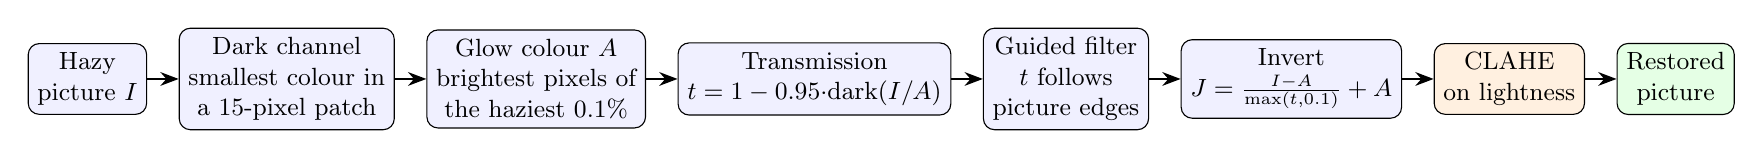
\begin{tikzpicture}[node distance=4mm]
\node[box](a){Hazy\\picture $I$};
\node[box,right=of a](b){Dark channel\\smallest colour in\\a 15-pixel patch};
\node[box,right=of b](c){Glow colour $A$\\brightest pixels of\\the haziest 0.1\%};
\node[box,right=of c](d){Transmission\\$t=1-0.95\cdot$dark$(I/A)$};
\node[box,right=of d](e){Guided filter\\$t$ follows\\picture edges};
\node[box,right=of e](f){Invert\\$J=\frac{I-A}{\max(t,0.1)}+A$};
\node[box,right=of f,fill=orange!12](g){CLAHE\\on lightness};
\node[box,right=of g,fill=green!10](h){Restored\\picture};
\foreach \x/\y in {a/b,b/c,c/d,d/e,e/f,f/g,g/h}{\draw[arr](\x)--(\y);}
\end{tikzpicture}}\caption{Guided DCP followed by CLAHE (``DCP then CLAHE''), the best single chain on real haze. The orange box is the added post-processing step.}\end{figure}
\begin{figure}[H]\centering\resizebox{\textwidth}{!}{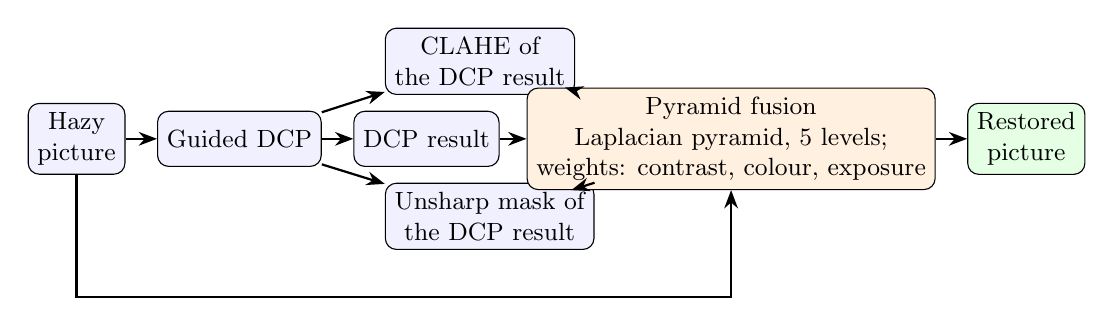
\begin{tikzpicture}[node distance=4mm]
\node[box](a){Hazy\\picture};
\node[box,right=of a](b){Guided DCP};
\node[box,above right=2mm and 8mm of b](c){CLAHE of\\the DCP result};
\node[box,right=of b](d){DCP result};
\node[box,below right=2mm and 8mm of b](e){Unsharp mask of\\the DCP result};
\node[box,right=26mm of b,fill=orange!12](f){Pyramid fusion\\Laplacian pyramid, 5 levels;\\weights: contrast, colour, exposure};
\node[box,right=of f,fill=green!10](g){Restored\\picture};
\draw[arr](a)--(b);\draw[arr](b)--(c);\draw[arr](b)--(d);\draw[arr](b)--(e);
\draw[arr](c)--(f);\draw[arr](d)--(f);\draw[arr](e)--(f);\draw[arr](a.south)|-([yshift=-6mm]e.south)-|(f.south);\draw[arr](f)--(g);
\end{tikzpicture}}\caption{\texttt{fusion\_dcp}: the original and three versions of the DCP result are blended, level by level, keeping at each place the version with the best contrast, colour and exposure.}\end{figure}
\begin{figure}[H]\centering\resizebox{\textwidth}{!}{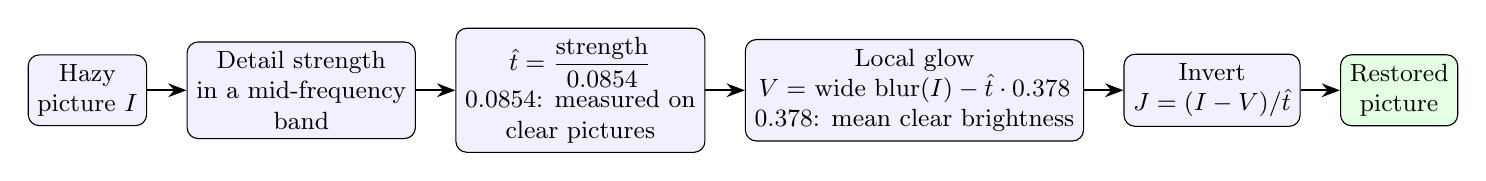
\begin{tikzpicture}[node distance=5mm]
\node[box](a){Hazy\\picture $I$};
\node[box,right=of a](b){Detail strength\\in a mid-frequency\\band};
\node[box,right=of b](c){$\hat t=\dfrac{\text{strength}}{0.0854}$\\0.0854: measured on\\clear pictures};
\node[box,right=of c](d){Local glow\\$V=$ wide blur$(I)-\hat t\cdot0.378$\\0.378: mean clear brightness};
\node[box,right=of d](e){Invert\\$J=(I-V)/\hat t$};
\node[box,right=of e,fill=green!10](f){Restored\\picture};
\foreach \x/\y in {a/b,b/c,c/d,d/e,e/f}{\draw[arr](\x)--(\y);}
\end{tikzpicture}}\caption{Haze removal by subtraction (\texttt{blind\_veil}, local form). No dark-channel assumption: it uses the frequency result that haze scales detail by $t$.}\end{figure}
\begin{figure}[H]\centering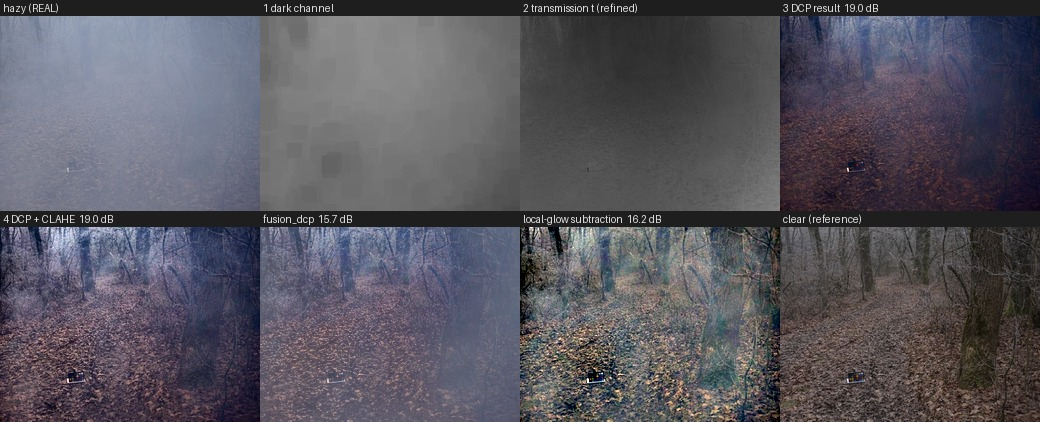
\includegraphics[width=.92\textwidth]{pipeline_haze.jpg}\caption{\REAL\ The haze pipelines on one real photo. Top: hazy photo; step 1 dark channel (bright = hazy); step 2 transmission $t$ (dark = thick haze); step 3 the DCP result (dark, blue cast). Bottom: DCP then CLAHE; fusion; local-glow subtraction; the clear photo.}\end{figure}

\needspace{9\baselineskip}
\paragraph{The longer chains, step by step.} A chain is only worth keeping if each step pays for itself. The figure shows the best haze chain after every step, with the PSNR under each picture. On the \SYN\ haze the whole chain gains 2.7 dB. On the \REAL\ photo (second row) equalisation alone makes it \emph{worse} (11.0 to 9.2 dB), CLAHE and DCP then recover it to 12.4: the later steps repair what the first one broke. The third row is the best real-haze chain, DCP then CLAHE.
\begin{figure}[H]\centering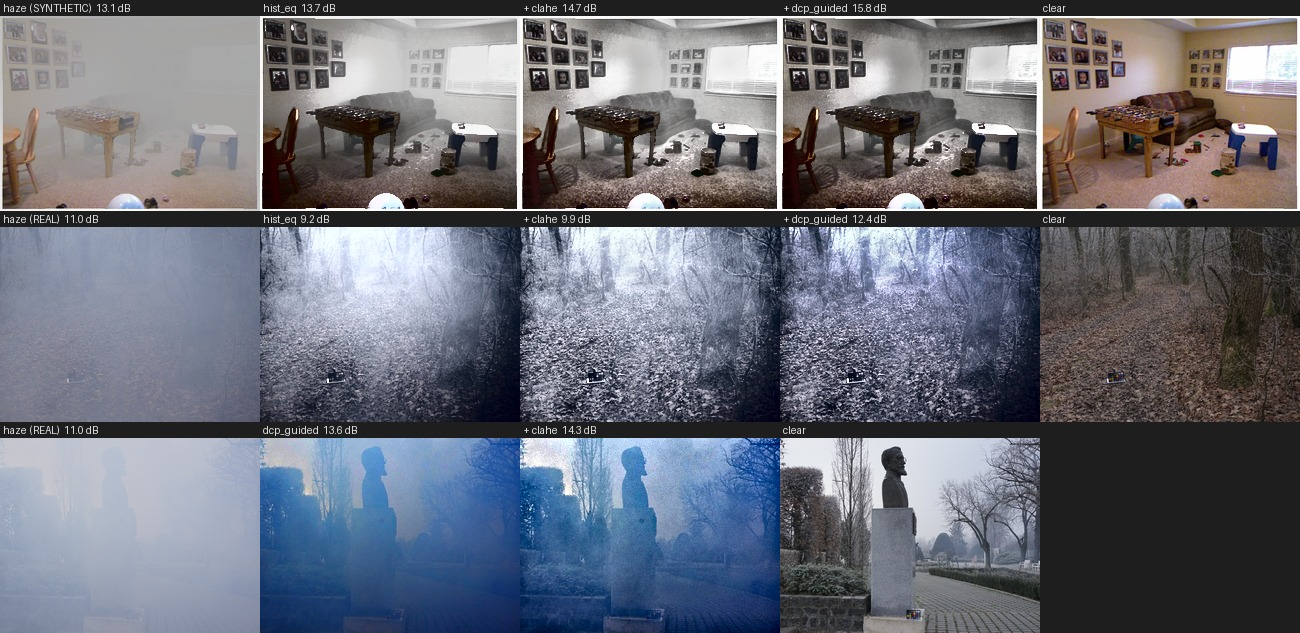
\includegraphics[width=.95\textwidth]{pipeline_haze_chain.jpg}\caption{The haze chain \texttt{hist\_eq > clahe > dcp\_guided} on \SYN\ haze (row 1) and on a \REAL\ photo (row 2); row 3: \REAL\ photo with \texttt{dcp\_guided > clahe}. The PSNR against the clear picture is in each caption.}\end{figure}

\needspace{9\baselineskip}
\paragraph{Local application (a wrapper that works with any method).}
\begin{figure}[H]\centering\resizebox{.95\textwidth}{!}{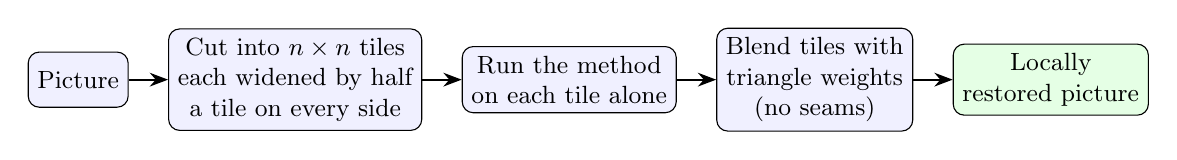
\begin{tikzpicture}[node distance=5mm]
\node[box](a){Picture};
\node[box,right=of a](b){Cut into $n\times n$ tiles\\each widened by half\\a tile on every side};
\node[box,right=of b](c){Run the method\\on each tile alone};
\node[box,right=of c](d){Blend tiles with\\triangle weights\\(no seams)};
\node[box,right=of d,fill=green!10](e){Locally\\restored picture};
\foreach \x/\y in {a/b,b/c,c/d,d/e}{\draw[arr](\x)--(\y);}
\end{tikzpicture}}\caption{Tile-wise application (Section~\ref{sec:local}). The variant with regions groups pixels by haze thickness (dark channel) or sharpness instead of cutting a grid.}\end{figure}

\needspace{9\baselineskip}
\paragraph{Water (open-sea style colour cast).}
\begin{figure}[H]\centering\resizebox{\textwidth}{!}{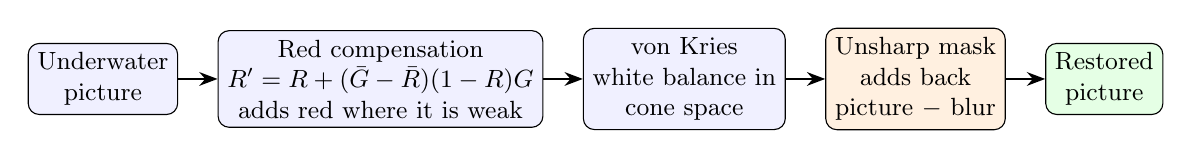
\begin{tikzpicture}[node distance=5mm]
\node[box](a){Underwater\\picture};
\node[box,right=of a](b){Red compensation\\$R'=R+(\bar G-\bar R)(1-R)G$\\adds red where it is weak};
\node[box,right=of b](c){von Kries\\white balance in\\cone space};
\node[box,right=of c,fill=orange!12](d){Unsharp mask\\adds back\\picture $-$ blur};
\node[box,right=of d,fill=green!10](e){Restored\\picture};
\foreach \x/\y in {a/b,b/c,c/d,d/e}{\draw[arr](\x)--(\y);}
\end{tikzpicture}}\caption{Best chain on synthetic water (\texttt{red\_comp}, \texttt{von\_kries}; the unsharp step is the searched third step). UDCP differs from DCP only in using green and blue for the dark channel, because red is already gone.}\end{figure}
\begin{figure}[H]\centering\includegraphics[width=.92\textwidth]{pipeline_water.jpg}\caption{The chain \texttt{red\_comp > von\_kries > unsharp} on four kinds of water. Row 1: \SYN\ open-sea water (+3.1 dB). Row 2: \SYN\ milky water (worse: 14.7 to 14.2 dB). Row 3: \REAL\ tank water (worse: 18.2 to 16.7 dB). Row 4: \REAL\ ocean photo (no reference, so no score). Where the water really has a colour cast (rows 1 and 4) the first two steps remove it; where it is milky (rows 2 and 3) there is no cast to remove, and the steps only change the colours.}\end{figure}

\needspace{9\baselineskip}
\paragraph{Glass.}
No method beat doing nothing on raindrops. The glass methods tried are DCP variants that change one assumption each: \texttt{dcp\_near\_global} (one almost constant $t$ for the whole picture, because the film is on the pane and not at varying distance), \texttt{dcp\_local\_airlight} (glow colour estimated region by region, for an uneven film), and \texttt{flat\_field} (divide out a slowly varying brightness).
\begin{figure}[H]\centering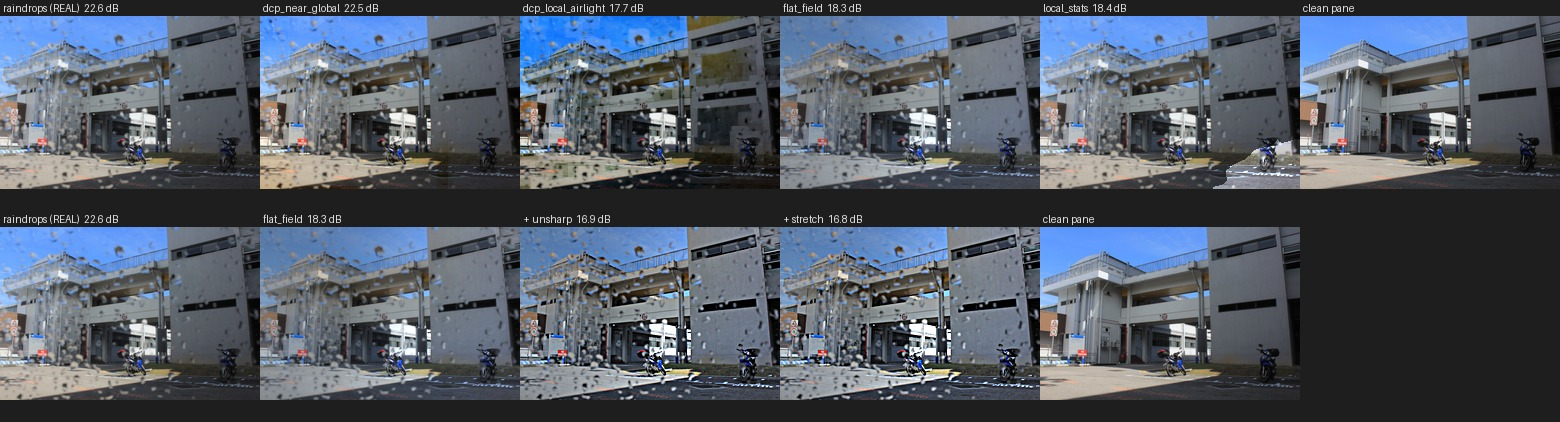
\includegraphics[width=.92\textwidth]{pipeline_glass.jpg}\caption{\REAL\ Raindrops. Row 1: the glass-specific methods, each applied to the original, and the clean pane. Row 2: a chain \texttt{flat\_field > unsharp > stretch}; each step lowers the PSNR (22.6, 18.3, 16.9, 16.8 dB). The methods change the colours and brightness of the whole picture but cannot recover what the drops hide, which is why the best chain for glass is the empty one.}\end{figure}
\paragraph{Stacked media.}
\begin{figure}[H]\centering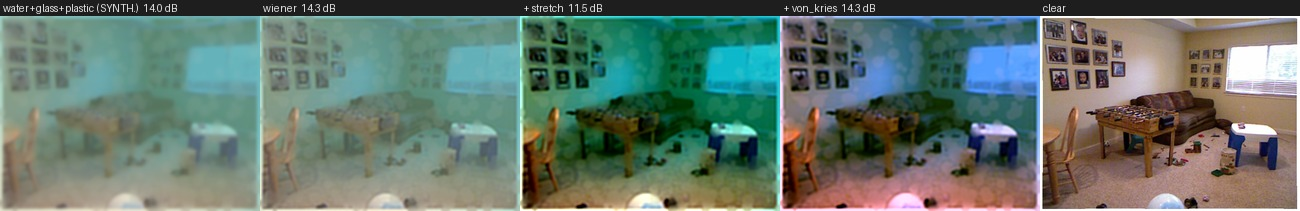
\includegraphics[width=.95\textwidth]{pipeline_stack.jpg}\caption{\SYN\ A picture seen through water, then glass with raindrops, then plastic, restored by the searched chain \texttt{wiener > stretch > von\_kries}. The middle step makes the picture worse (14.3 to 11.5 dB) and the last step brings it back to 14.3: the chain ends where its first step already was, so the gain over doing nothing (14.0 dB) is small.}\end{figure}

\needspace{9\baselineskip}
\paragraph{Plastic.}
\begin{figure}[H]\centering\resizebox{\textwidth}{!}{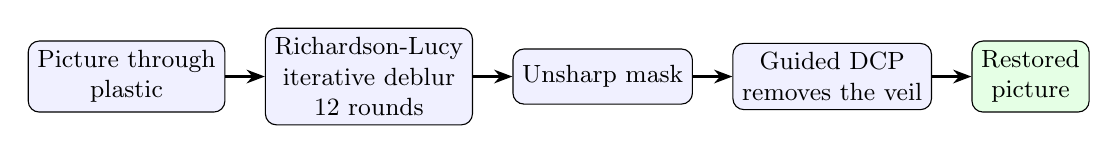
\begin{tikzpicture}[node distance=5mm]
\node[box](a){Picture through\\plastic};
\node[box,right=of a](b){Richardson-Lucy\\iterative deblur\\12 rounds};
\node[box,right=of b](c){Unsharp mask};
\node[box,right=of c](d){Guided DCP\\removes the veil};
\node[box,right=of d,fill=green!10](e){Restored\\picture};
\foreach \x/\y in {a/b,b/c,c/d,d/e}{\draw[arr](\x)--(\y);}
\end{tikzpicture}}\caption{Best chain on synthetic plastic. The best single step is a plain linear contrast stretch.}\end{figure}
\begin{figure}[H]\centering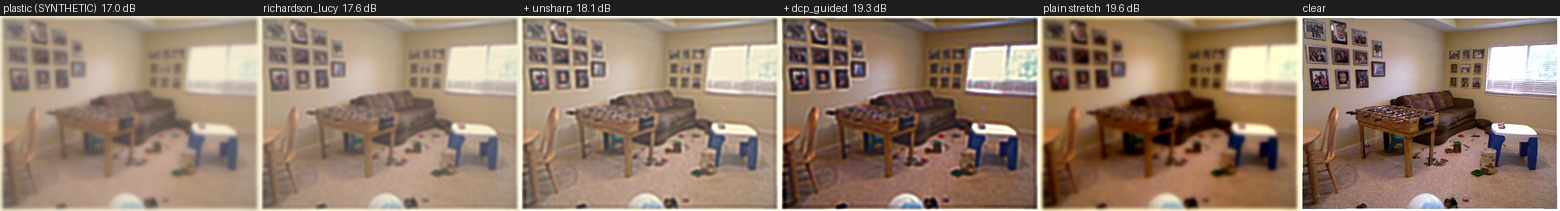
\includegraphics[width=.95\textwidth]{pipeline_plastic.jpg}\caption{\SYN\ Plastic, after each step of the chain (PSNR in each caption), the plain stretch, and the clear original. On this picture the chain gains +2.3 dB and the single stretch step +2.6 dB.}\end{figure}

\needspace{9\baselineskip}
\paragraph{How the best chains were found.}
\begin{figure}[H]\centering\resizebox{\textwidth}{!}{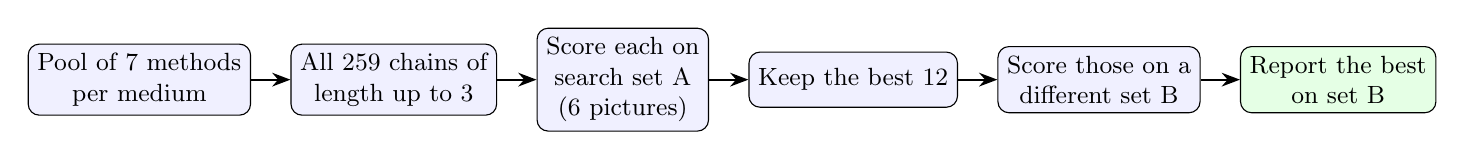
\begin{tikzpicture}[node distance=5mm]
\node[box](a){Pool of 7 methods\\per medium};
\node[box,right=of a](b){All 259 chains of\\length up to 3};
\node[box,right=of b](c){Score each on\\search set A\\(6 pictures)};
\node[box,right=of c](d){Keep the best 12};
\node[box,right=of d](e){Score those on a\\different set B};
\node[box,right=of e,fill=green!10](f){Report the best\\on set B};
\foreach \x/\y in {a/b,b/c,c/d,d/e,e/f}{\draw[arr](\x)--(\y);}
\end{tikzpicture}}\caption{The step-order search. The best chain is chosen on one set and judged on another, so the result is not a lucky fit.}\end{figure}
\begin{table}[H]\centering\small
\begin{tabular}{p{1.5cm}p{4.6cm}p{9.2cm}}\toprule
Medium & Best chain found & Assumption each step makes\\\midrule
Haze & hist\_eq, CLAHE, guided DCP (synthetic); DCP, CLAHE (real) & Dark channel: some pixel in each patch is dark. CLAHE: contrast is lost locally, not just globally.\\
Water & red compensation, von Kries (+ unsharp) & Red is the colour lost; the average colour of the scene should be neutral.\\
Glass & none & Raindrops hide patches of the scene; no whole-picture step brings them back.\\
Plastic & Richardson-Lucy, unsharp, guided DCP (best single: stretch) & The blur is Gaussian and known; the rest is a dimming plus a milky veil.\\\bottomrule
\end{tabular}\caption{Summary of the pipelines. Scores are in Section~\ref{sec:synthetic}--\ref{sec:compare}.}\end{table}

\subsection{How we score}
\textbf{PSNR} (in dB, higher is better) says how close the repaired picture is to the clean one pixel by pixel; \textbf{SSIM} (0 to 1) says how well the structure matches; \textbf{CIEDE2000} (lower is better) measures colour error. ``\emph{None}'' means: do nothing to the spoiled picture. A method that scores below ``none'' makes things worse.

%--------------------------------------------------------------------
\section{Results on made-up pictures \SYN}
\label{sec:synthetic}
Here the clean answer is exact. We show the \textbf{calibrated} versions of haze and glass (settings tuned to look like the real thing; Section~\ref{sec:compare} explains why and what it changed). Water and plastic are the same in both versions.

\subsection{Which method is best?}
\begin{table}[H]\centering\scriptsize
\begin{minipage}{.48\textwidth}\centering\textbf{haze \SYN}\\\tablein{matched_haze}\end{minipage}\hfill
\begin{minipage}{.48\textwidth}\centering\textbf{water \SYN}\\\tablein{matched_water}\end{minipage}\\[6pt]
\begin{minipage}{.48\textwidth}\centering\textbf{glass (raindrops) \SYN}\\\tablein{matched_glass}\end{minipage}\hfill
\begin{minipage}{.48\textwidth}\centering\textbf{plastic \SYN}\\\tablein{matched_plastic}\end{minipage}
\caption{\SYN\ The best methods per medium (PSNR averaged over the made-up pairs; ``vs none'' is the gain over doing nothing).}\end{table}

Plain reading of the table:
\begin{itemize}
\item \textbf{Haze:} histogram methods lead; DCP is barely better than nothing. (With our \emph{original} hand-made haze, DCP was clearly best. That difference is the main story of Section~\ref{sec:compare}.)
\item \textbf{Water:} a colour correction (von Kries) wins, because water mostly shifts colours. (On real tank water nothing beats doing nothing; see Section~\ref{sec:realwater}.)
\item \textbf{Glass:} nothing beats ``none''. Raindrops replace patches of the scene; no global operation can bring those patches back.
\item \textbf{Plastic:} a plain contrast stretch wins; plastic is mostly a dimming, which a stretch undoes.
\end{itemize}

\begin{figure}[H]\centering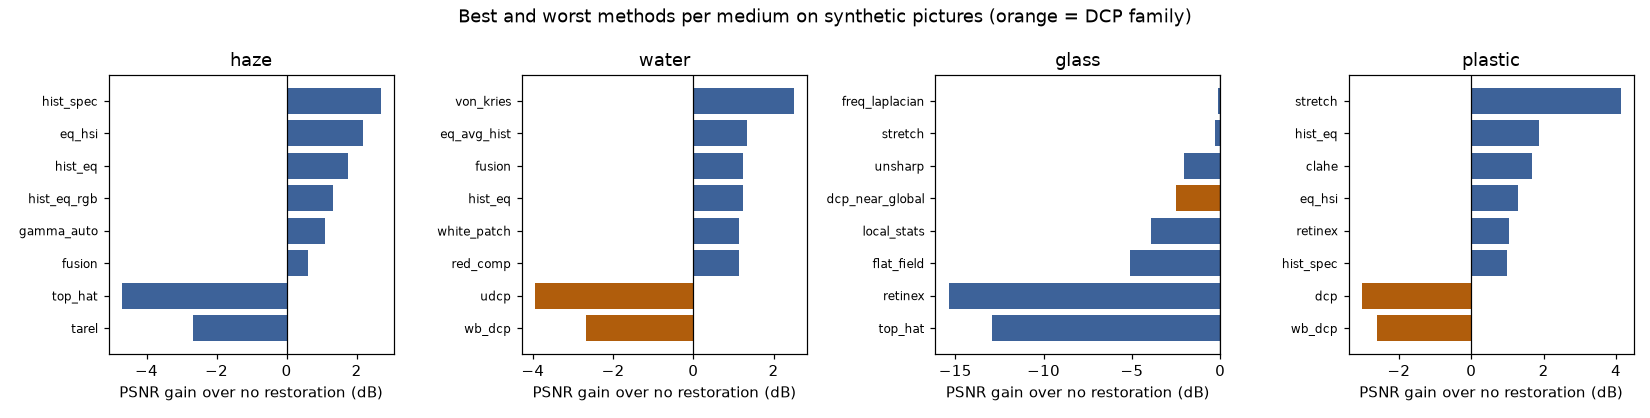
\includegraphics[width=\textwidth]{report_gain_over_none.png}\caption{\SYN\ Gain over doing nothing, per method and medium (blue bars help, red hurt).}\end{figure}

\subsection{What the repairs look like}
\begin{figure}[H]\centering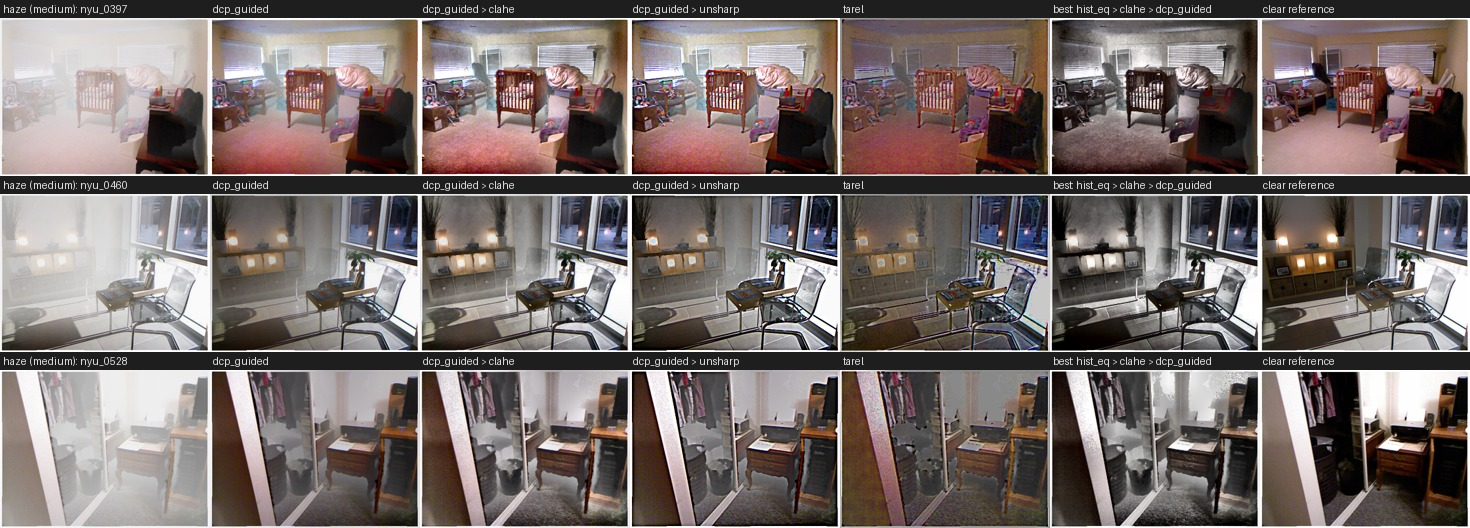
\includegraphics[width=.92\textwidth]{report_ba_haze.jpg}\caption{\SYN\ Haze. Each row is one picture: spoiled, several repairs, and the clean original on the right.}\end{figure}
\begin{figure}[H]\centering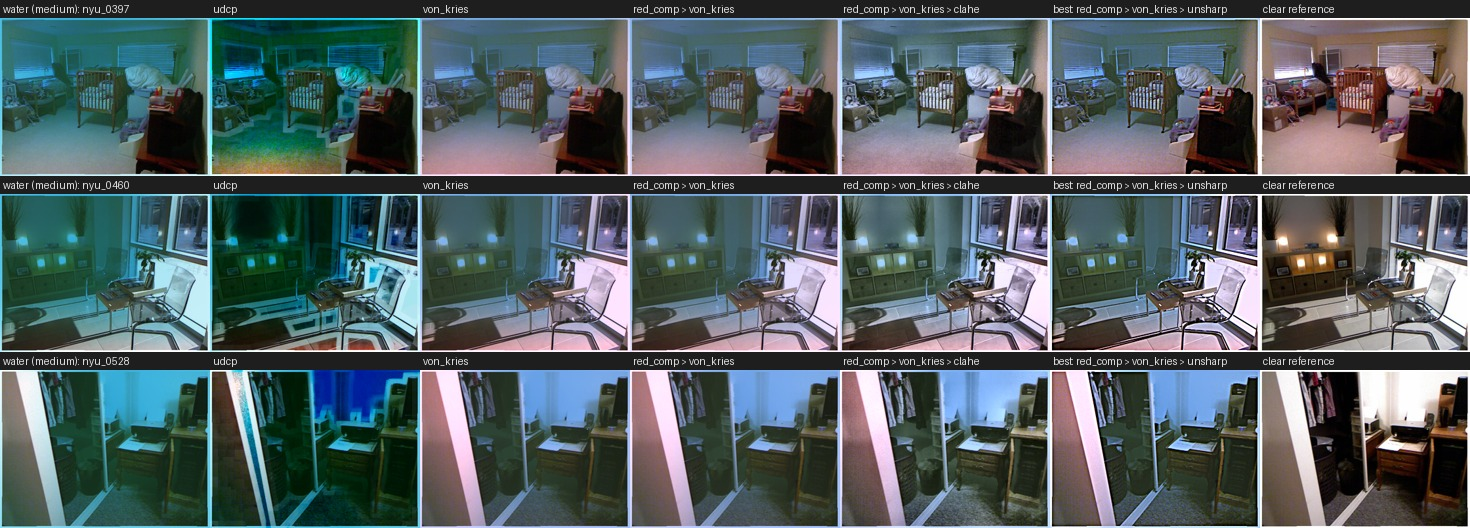
\includegraphics[width=.92\textwidth]{report_ba_water.jpg}\caption{\SYN\ Water, same layout.}\end{figure}

\subsection{Does the order of steps matter?}
We tried every chain of up to three steps from a short list, choosing the best on one set of pictures and checking it on a \emph{different} set, so the result is not luck.
\begin{table}[H]\centering\scriptsize\tablein{pipelines_verify}\caption{\SYN\ Best chain per medium on the held-out pictures, against DCP alone and doing nothing. \texttt{A > B} means run A first, then B on its output.}\end{table}
\begin{itemize}
\item \textbf{Yes, order matters}, by up to 3.1 dB between the best and worst order of the same steps.
\item \textbf{Haze:} a contrast chain \emph{before} DCP beats DCP alone (13.66 against 12.86 dB). So \textbf{something does beat DCP}, but only by a modest amount.
\item \textbf{Water:} red-channel compensation then von Kries, +5.0 dB over DCP (18.03 against 13.05).
\item \textbf{Plastic:} Richardson-Lucy deblur, sharpen, then DCP.
\end{itemize}
Post-processing is not free: histogram equalisation after gray-world helps haze (+3.8 dB) but hurts when applied after DCP (-1.5 dB).
\begin{figure}[H]\centering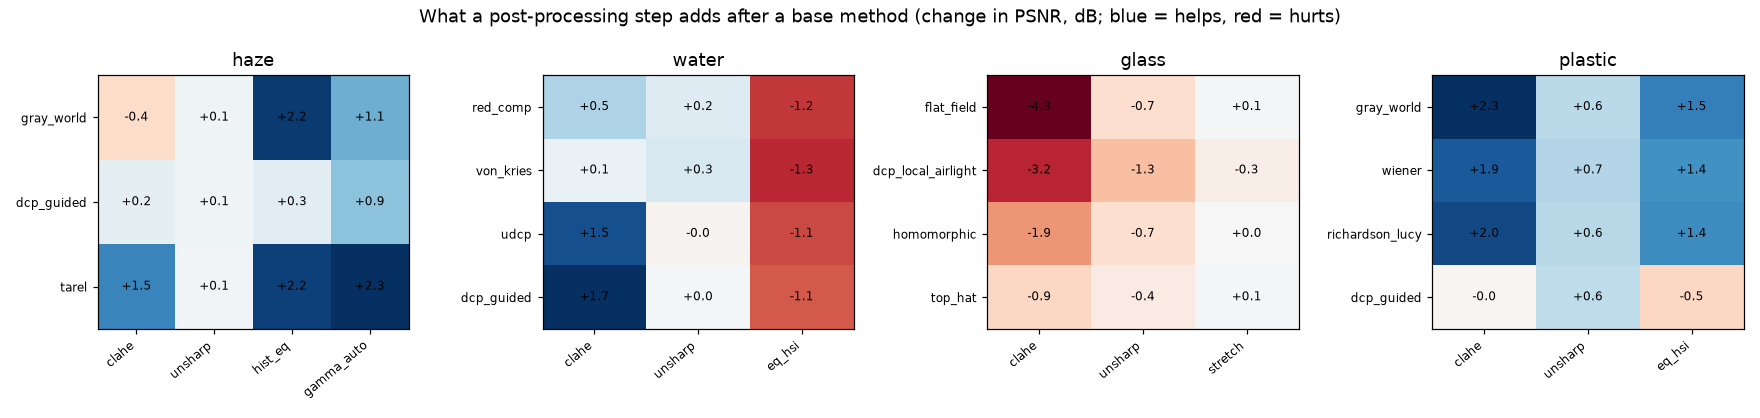
\includegraphics[width=\textwidth]{report_postprocessing.png}\caption{\SYN\ What an extra step adds after a base method (change in PSNR; blue helps, red hurts).}\end{figure}

\subsection{Stacked media}
\begin{figure}[H]\centering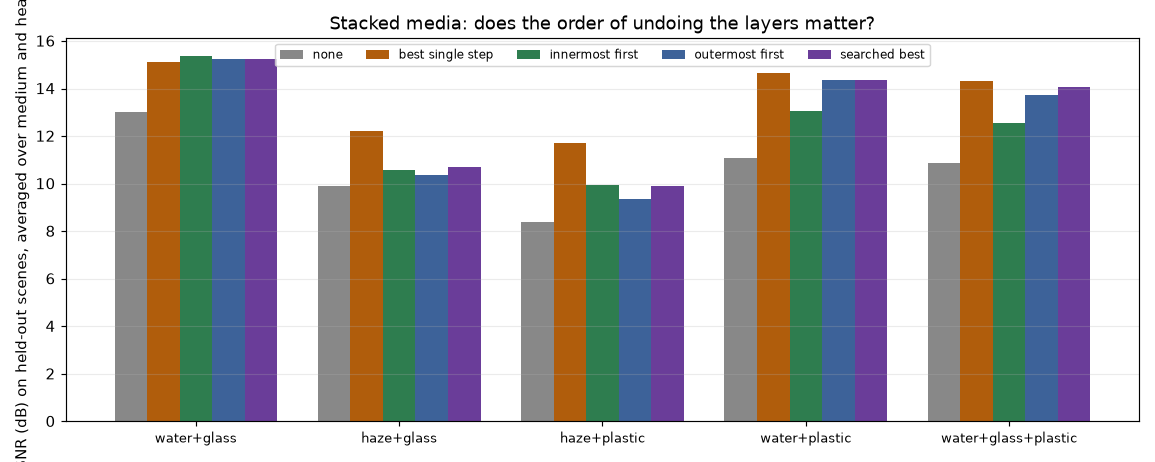
\includegraphics[width=.8\textwidth]{stacked_summary.png}\caption{\SYN\ Two or three media stacked, with different orders of undoing them. With the calibrated glass the order matters little and not consistently.}\end{figure}

%--------------------------------------------------------------------
\section{Results on real pictures \REAL}\label{sec:real}
Now the real thing, where no model is involved.
\begin{table}[H]\centering\scriptsize
\begin{minipage}{.48\textwidth}\centering\textbf{real haze, 185 pairs \REAL}\\\tablein{real_haze}\end{minipage}\hfill
\begin{minipage}{.48\textwidth}\centering\textbf{real raindrops, 58 pairs \REAL}\\\tablein{real_glass}\end{minipage}
\caption{\REAL\ Best methods on real pictures: all 185 haze pairs and all 58 raindrop pairs. (A first version used only 36 pictures of each: the top two haze methods swapped places, a tie within 0.2 dB, and the raindrop result did not change.)}\end{table}
\begin{itemize}
\item \textbf{Real haze:} The two best are \emph{fusion after DCP} (14.76 dB) and \emph{DCP followed by CLAHE} (14.61 dB); doing nothing scores 12.00. DCP followed by CLAHE beats DCP alone by +0.86 dB (standard error 0.14; better on 138 of 185 pairs; SSIM +0.094). DCP alone leaves a dark picture with a blue cast; the contrast step brings brightness back.
\item \textbf{Real raindrops:} again nothing helps (``none'' scores highest, 24.02 dB; the best method, a frequency-domain Laplacian, is 0.11 dB lower and better on only 12 of 58 pairs).
\end{itemize}
\begin{figure}[H]\centering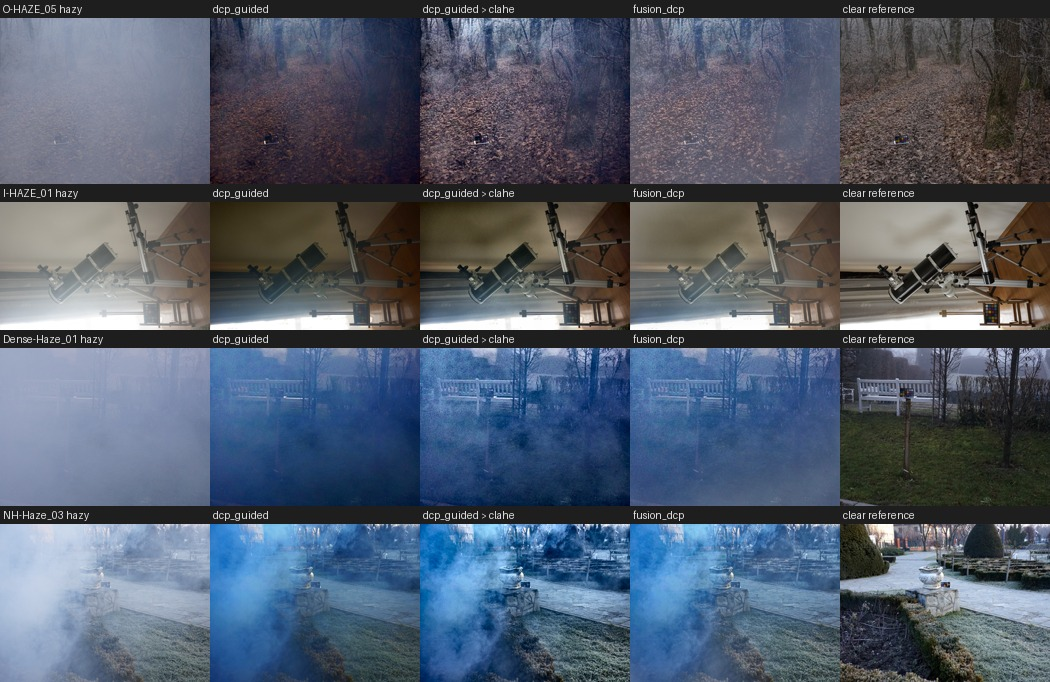
\includegraphics[width=.92\textwidth]{report_ba_real_haze.jpg}\caption{\REAL\ Haze. Hazy photo, three repairs, clean photo (right).}\end{figure}

\subsection{Real underwater pictures \REAL}
\label{sec:realwater}
Two kinds of real underwater data.

\textbf{TUB, paired tank photos.} Objects sit in a water tank; milk is added in 10 steps while camera and objects stay fixed. The least turbid picture of each view is our reference. It is nearly clear (a few NTU, a unit of turbidity), not perfectly clear, so scores are against a nearly clear reference. Two cautions: the turbidity is milky scattering (brown-grey haze, much like fog), not the blue-green colour cast of the open sea; and the camera adjusts its exposure between steps, which PSNR counts as error.
\begin{table}[H]\centering\scriptsize
\begin{minipage}{.48\textwidth}\centering\textbf{water methods, 120 TUB pairs \REAL}\\\tablein{real_water_tub}\end{minipage}\hfill
\begin{minipage}{.48\textwidth}\centering\textbf{haze methods (DCP and others), same pairs \REAL}\\\tablein{real_water_tub_hazemethods}\end{minipage}
\caption{\REAL\ Repair of real turbid tank water, averaged over 120 pairs (40 per turbidity band).}\end{table}
\begin{figure}[H]\centering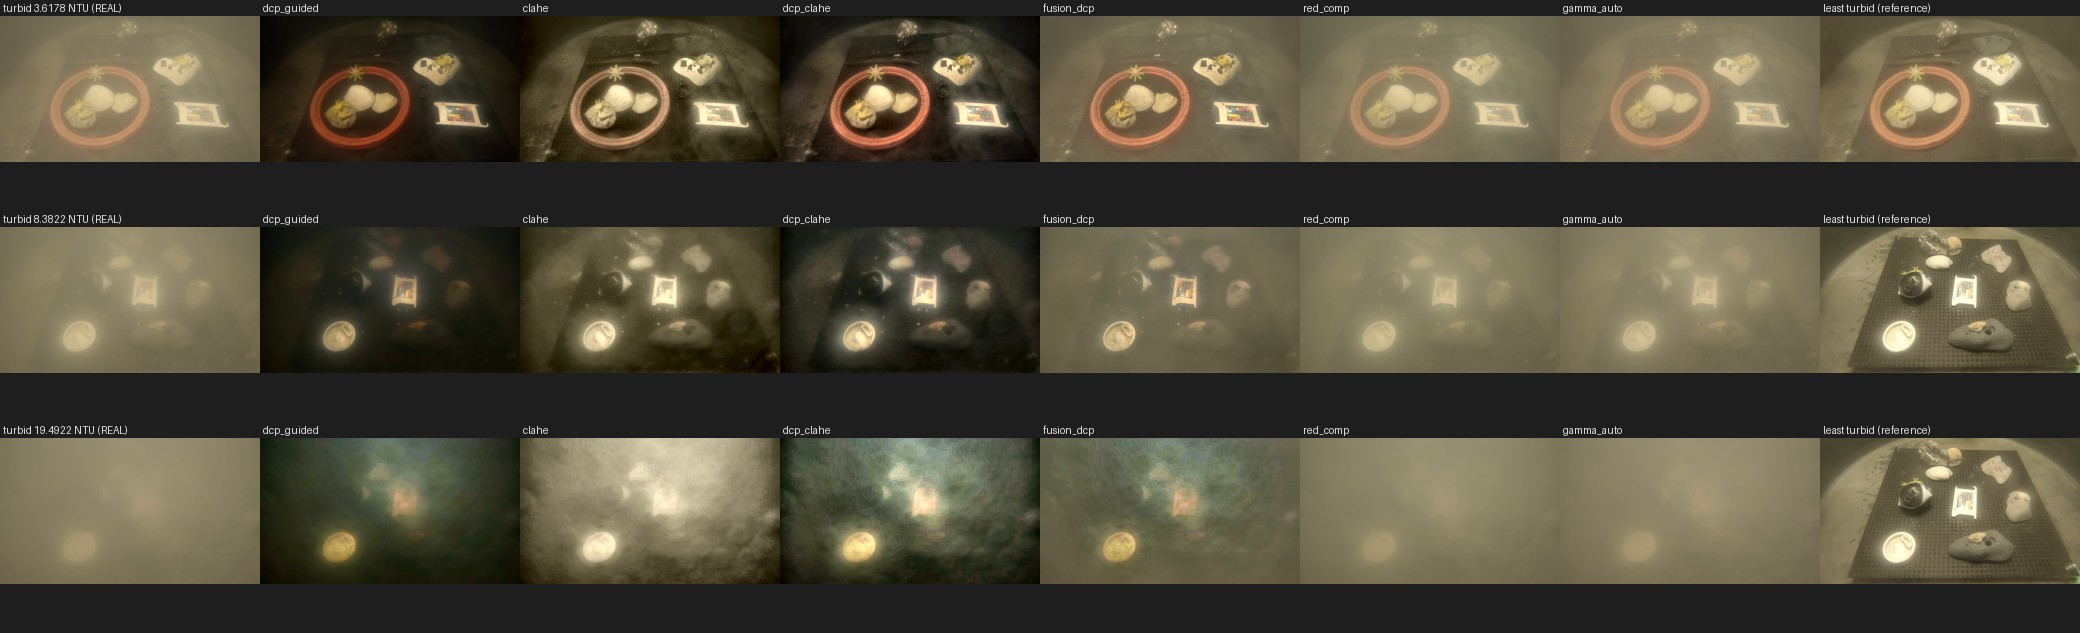
\includegraphics[width=\textwidth]{report_ba_tub.jpg}\caption{\REAL\ Paired tank water. Rows: mild, medium, heavy turbidity. Left: turbid picture; middle: repairs; right: the least turbid picture of the same view.}\end{figure}
\textbf{Reading.} Nothing beats doing nothing by more than 0.1 dB. DCP makes things much worse (11.45 dB against 18.72 for nothing): it darkens the picture and shifts the colours. CLAHE scores 15.83 and DCP followed by CLAHE 13.98, both worse than doing nothing. In the pictures the repairs do bring out colour and contrast (DCP, CLAHE) but they also darken the scene and amplify the noise, and none of them returns the detail that is lost: at heavy turbidity almost nothing is left to recover.

\textbf{UIEB, ocean and reef photos.} No clean twin exists, so we can only look at them and use reference-free scores.
\begin{figure}[H]\centering\includegraphics[width=\textwidth]{report_ba_uieb.jpg}\caption{\REAL\ Ocean and reef photos (no clean reference). Left: original; then six repairs. Colour correction (red compensation, von Kries) brings back warm colours; \texttt{wb\_dcp} and \texttt{fusion} over-correct and turn the seabed red; UDCP turns the scene dark blue.}\end{figure}
On these photos the problem is mostly \emph{colour}, and the colour methods work visibly better than DCP-style methods, in line with the synthetic water results. We cannot put a number on it, because reference-free scores disagree with each other (UCIQE prefers UDCP and stretch, while the remaining colour cast prefers equalised-average-histogram, fusion and von Kries; see the project log, finding F55).

%--------------------------------------------------------------------
\section{Can made-up pictures stand in for real ones?}
\label{sec:compare}
We compared \SYN\ with \REAL\ in seven ways, from the simplest to the most demanding.

\subsection{Test 1: do they look statistically alike?}
For each spoiled picture we measure five simple things against its clean twin: how much the darkest values rise (\emph{dark shift}), how much contrast is lost (\emph{contrast ratio}, 1 = unchanged), how much brighter it is, how much detail remains (\emph{sharpness ratio}), and the share of the picture that changed.
\begin{table}[H]\centering\scriptsize\tablein{signature_compare}\caption{\BOTH\ How much each degradation changes the picture. The closer a synthetic row is to the real row above it, the better the match.}\end{table}
\textbf{Reading.} Our original haze was too bright and too sharp (contrast ratio 0.65--0.81 against 0.40--0.70 in real fog; sharpness 0.34--0.72 against 0.13--0.40). The calibrated haze is much closer (sharpness 0.17 against 0.13 for heavy, contrast 0.40 against 0.40). Fitting the haze model to real pairs gave a glow of brightness $A\approx0.60$--$0.70$, not our original $0.92$. Real raindrops barely change brightness or contrast (ratio near 0.9), so a veil model is wrong for them; droplets-only fits.

\subsection{Test 2: do the same methods win?}
For every method we plot its score on synthetic pictures against its score on real ones. If the models were perfect, the dots would sit on the dashed line, and a high-scoring method on one side would be high-scoring on the other.
\begin{figure}[H]\centering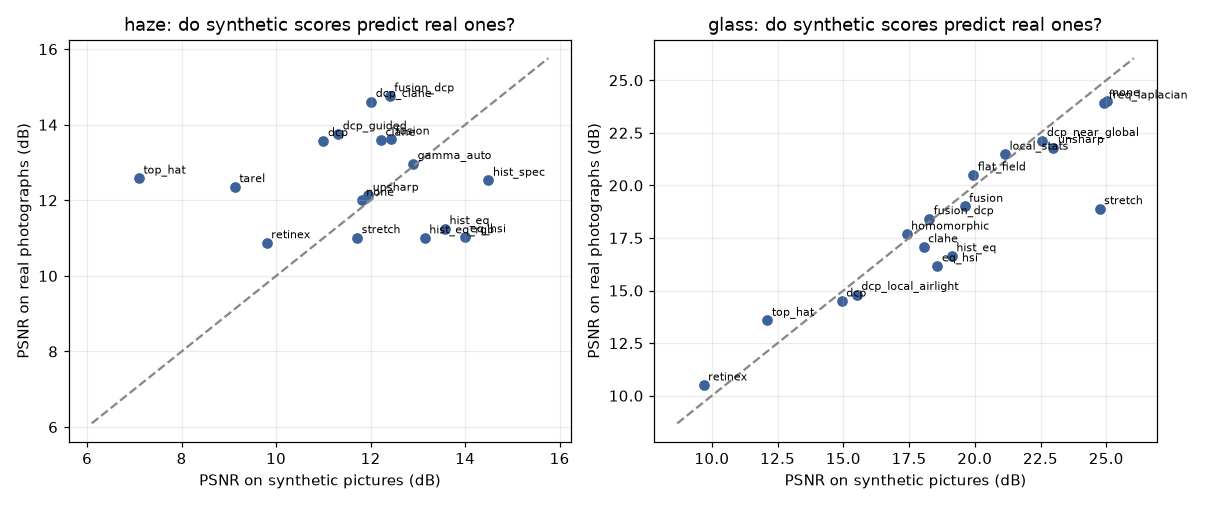
\includegraphics[width=\textwidth]{report_synthetic_vs_real.png}\caption{\BOTH\ Each dot is one method. Left: haze (synthetic is the calibrated version). Right: raindrops on glass.}\end{figure}
\begin{itemize}
\item \textbf{Glass:} the dots follow the line closely. Methods rank almost the same (Spearman correlation 0.92 on 12 scenes, 0.85 on 90). The one clear outlier is \emph{stretch}, which scores 24.7 dB on synthetic and 18.6 dB on real raindrops.
\item \textbf{Haze:} the dots are scattered (correlation $-0.04$ on the 12 scenes of this figure; with 90 scenes it is +0.30, see Test 7). Histogram methods (\texttt{hist\_spec}, \texttt{eq\_hsi}) score well on synthetic and poorly on real; the DCP-plus-CLAHE family scores best on real and middling on synthetic.
\end{itemize}

\begin{table}[H]\centering\scriptsize\tablein{before_after_presets}\caption{\BOTH\ Original hand-chosen presets against calibrated ones. Rank agreement is the correlation between how methods rank on synthetic and on real pictures (1 = identical, 0 = unrelated).}\end{table}

\subsection{Test 3: what did calibration change?}
We tuned the settings of haze and glass to look like the real thing, then reran the experiments. The old results are kept in \texttt{results\_original\_presets/}.
\begin{itemize}
\item \textbf{With the original haze,} DCP looked excellent (+5.1 dB over nothing). On calibrated haze and on real haze it is weak. \emph{The original settings flattered DCP.}
\item \textbf{With the original glass,} a plain stretch gained +10 dB. On raindrops (calibrated and real), nothing helps. \emph{The original settings flattered stretch.}
\item \textbf{Glass agreement rose} from 0.53 to 0.92.
\item \textbf{Haze agreement got worse with calibration.} Against all 185 real pairs, the original haze ranks the methods at +0.57 and the calibrated haze at $-0.04$ (12 scenes each); Test 7 repeats this on 90 scenes (+0.57 against +0.30). Calibration matched the \emph{statistics} in Test 1, not the \emph{ranking}.
\end{itemize}

\subsection{Test 4: remove the scene as an excuse}
In Tests 2 and 3 the synthetic pictures show indoor rooms and the real haze shows outdoor gardens, so a mismatch could simply be the scenery. Test 4 takes each real pair, degrades its \emph{own clean picture} with our model, and compares the real spoiled picture with its synthetic twin.
\begin{table}[H]\centering\scriptsize\tablein{scene_matched}\caption{\BOTH\ Same scene, real degradation against synthetic twin. The model for haze uses the strength fitted on the other half of the same dataset.}\end{table}
Now the rankings agree for \textbf{haze (+0.81)} and \textbf{glass (+0.99)}, and a method that helps a real picture also tends to help its twin (per-picture correlation 0.54 for haze, 0.93 for glass). So the model itself is reasonable for haze and good for glass when scene and haze strength are the same as in the real picture. Test 7 shows that this does not carry over to other scenes: with other scenes (indoor or outdoor) the ranking agreement is only +0.1 to +0.5.
\begin{figure}[H]\centering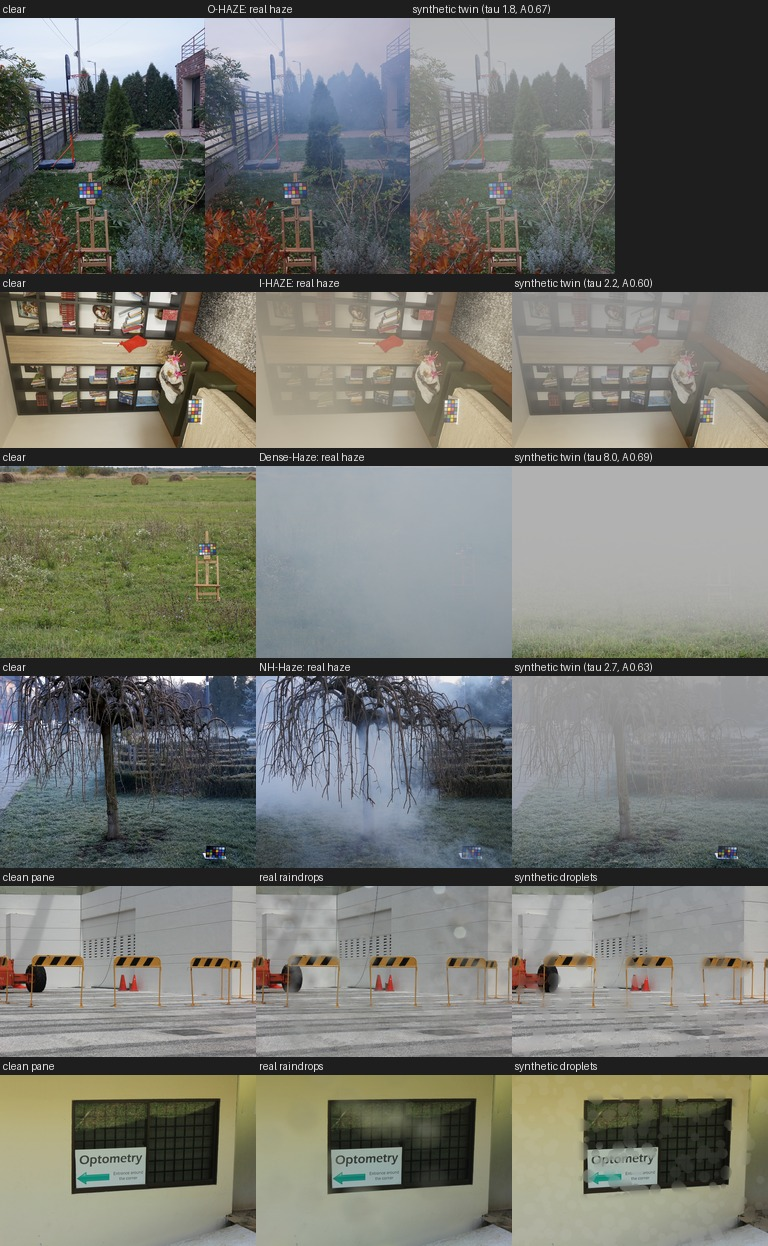
\includegraphics[width=.9\textwidth]{scene_matched_examples.jpg}\caption{\BOTH\ Clean picture, the real spoiled picture, and our synthetic twin of it.}\end{figure}

\subsection{Test 5: water, now with real pairs}
The real tank pairs let us do the same ranking test for water.
\begin{table}[H]\centering\scriptsize\tablein{water_tub_agreement}\caption{\BOTH\ Do the 17 water methods rank alike on real tank water and on synthetic water? Rank agreement is the correlation between the two rankings.}\end{table}
Agreement is moderate (+0.3 to +0.4) and falls with turbidity. The real winners are different from the synthetic ones: on synthetic water von Kries wins by a large margin; on real tank water nothing beats doing nothing. One plausible reason: milky tank water is scattering, close to the haze model, not the colour absorption our water model emphasises. Test 6 tests exactly that.

\subsection{Test 6: synthetic water with milky scattering \SYN}
\label{sec:milky}
We built a second synthetic water, \emph{milky water}, that matches the tank rather than the open sea. Open-sea water absorbs red first. Milk in a tank mainly \emph{scatters} all colours alike, so the picture fades towards a light brown-grey, like fog. Its equation is the haze equation with three changes: the same $\beta$ for all colours, the glow colour measured on the most turbid tank pictures (about 0.55, 0.52, 0.41 in red, green, blue), and an optional blur, because forward scattering smears the scene (in the tank, detail was lost faster than contrast). We chose the density $\beta$ and the blur for each turbidity band so that the five signature numbers of Test 1 match the real tank pairs.
\begin{figure}[H]\centering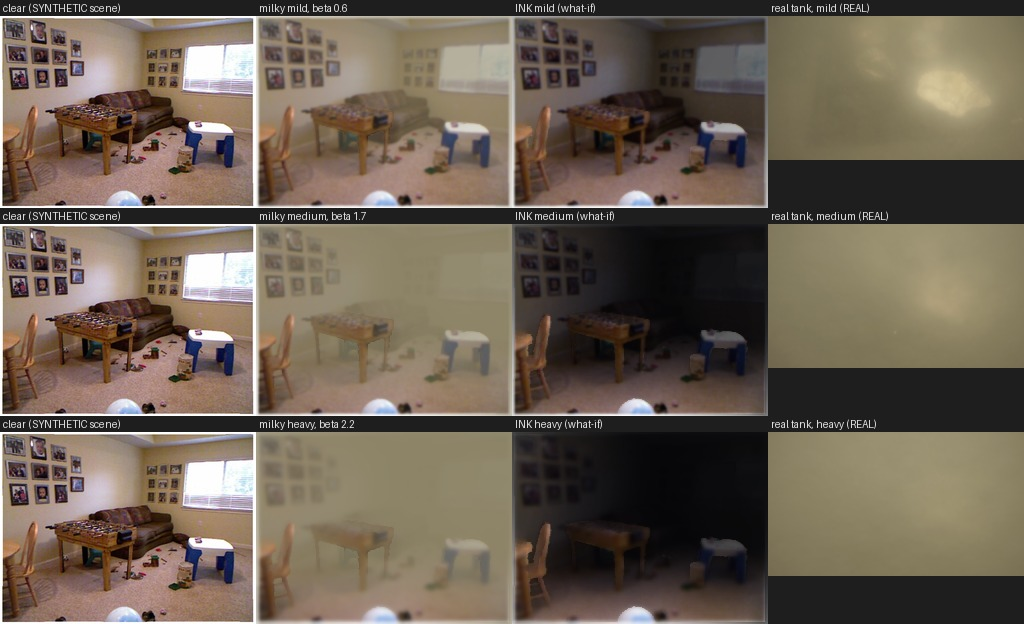
\includegraphics[width=.92\textwidth]{milky_examples.jpg}\caption{\BOTH\ Left to right: a clear synthetic scene, the same scene with calibrated milky water, the same density with a black cloud (the \emph{ink} what-if, next subsection), and a real tank picture of the same turbidity band (a different scene). Rows: mild, medium, heavy.}\end{figure}
\begin{table}[H]\centering\scriptsize\tablein{milky_signature}\caption{\BOTH\ How much each degradation changes the picture, real tank against calibrated synthetic milky water. Contrast and sharpness ratio: 1 = unchanged.}\end{table}
The match is only fair (the signature distance stays around 0.65 to 0.72 real spreads): our milky water fades the picture evenly, whereas the real tank had bright patches from the lamp and uneven light. Even so, the test result moved in the right direction.
\begin{table}[H]\centering\scriptsize\tablein{milky_agreement}\caption{\BOTH\ Rank agreement (correlation) between the real tank result and each synthetic water. ``Water methods'' are the 17 colour-oriented methods, ``haze methods'' the 17 DCP-family methods. The original water was only run with the water methods.}\end{table}
\begin{table}[H]\centering\scriptsize\tablein{milky_milk}\caption{\SYN\ Milky synthetic water: the best methods barely beat doing nothing (calibrated, 12 scenes, three densities).}\end{table}
\textbf{Reading.}
\begin{itemize}
\item \textbf{The verdict now agrees.} On the original synthetic water the colour methods won by a lot (von Kries +2.5 dB over nothing). On milky synthetic water, as on the real tank, the best method beats doing nothing by under 0.5 dB, and DCP-style methods hurt (guided DCP 12.8 against 15.0 for nothing; on the real tank 11.5 against 18.7). The size of the DCP loss is smaller on the synthetic water than on the real one.
\item \textbf{The full ranking only improves a little.} Overall agreement stays at +0.41 for the water methods and reaches +0.43 for the haze methods (+0.60 in the mild band, about +0.2 in the medium and heavy bands). When nearly every method is within a dB of doing nothing, the ranking is decided by small differences and is hard to reproduce.
\end{itemize}

\subsection{Does milky water look like squid or octopus ink? \SYN}
\textbf{In what they share.} A cloud of ink in water is also a cloud of particles between the scene and the camera: it lets a fraction $t$ of the scene light through and adds light of its own. The same equation $I=tJ+A(1-t)$ describes it, and it spoils the picture in the same way, by hiding detail.

\textbf{In what differs.} Milk particles scatter light and absorb almost none, so the cloud glows (large $A$, light colour). Ink (mostly the dark pigment melanin) absorbs strongly, so the cloud is dark ($A$ close to zero) and the scene fades towards \emph{black} instead of white. Real ink is also a patchy plume that spreads and dissolves within seconds, not an even cloud, so a spatially uniform model is a rough picture of it at best.

To see what that difference does to a repair, we ran the same density as the milky water but with a near-black cloud ($A\approx0.02$). There is no real ink data, so this is a what-if, not a calibration.
\begin{table}[H]\centering\scriptsize\tablein{milky_ink}\caption{\SYN\ Ink what-if (black cloud, same densities as the milky water, 12 scenes). Compare with the milky table above.}\end{table}
Here repairs \emph{do} help: the best gains +2.1 dB over nothing (fusion), and CLAHE, white-patch and automatic gamma gain 1.7 to 2.0 dB, because a dark cloud mostly lowers brightness, which brightening methods undo. DCP still hurts (9.3 against 10.9 dB for nothing). A likely reason, not tested: DCP assumes a bright glow and the glow here is black, so it estimates the wrong glow. So milky and inky water share an equation but not a remedy.

\subsection{Test 7: more scenes, and outdoor scenes}
\label{sec:outdoor}
Two doubts remained: the haze numbers of Tests 2 and 3 use only 12 indoor rooms, and the real haze is outdoors. We repeated the haze comparison with more scenes and a different kind of scene:
\begin{itemize}
\item \textbf{90 indoor rooms} (NYU), both the original and the calibrated haze;
\item \textbf{100 outdoor pictures} from RESIDE-SOTS, which comes with clear scenes and haze made by its own authors (so it tests the scene type but not our haze model).
\end{itemize}
\begin{table}[H]\centering\scriptsize\tablein{outdoor_haze}\caption{\SYN\ Rank agreement with real haze over the 17 haze methods, and the winners. All pictures here are synthetic; ``real haze'' is the reference of all 185 real pairs (best: fusion after DCP 14.76 dB; DCP then CLAHE 14.61; guided DCP 13.75; none 12.00).}\end{table}
\begin{figure}[H]\centering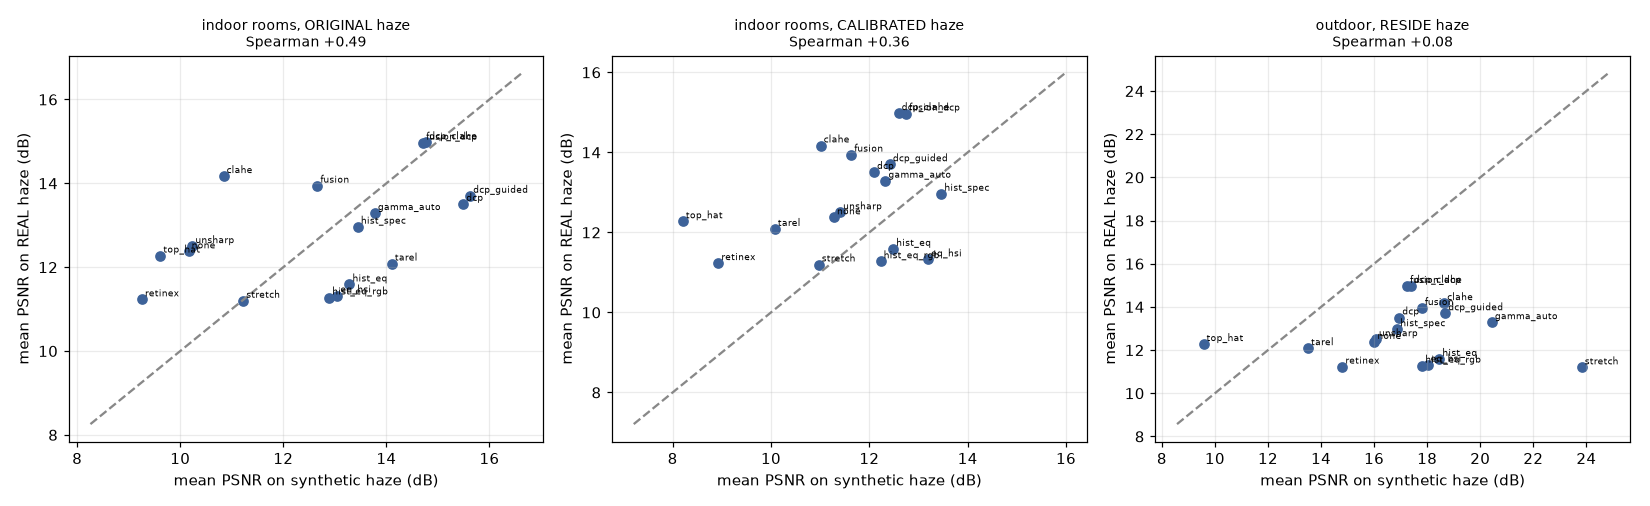
\includegraphics[width=.95\textwidth]{outdoor_haze.png}\caption{\BOTH\ Synthetic against real PSNR per method, for the three sets of synthetic haze.}\end{figure}
\begin{itemize}
\item \textbf{Twelve scenes are noisy for the calibrated haze.} Drawing 12-scene subsets from the 90 gives rank agreements from $-0.06$ to +0.55 (90\% of draws, calibrated haze) and +0.51 to +0.63 (original haze).
\item \textbf{Calibration made the ranking of haze worse.} On 90 scenes the original haze agrees at +0.57 and the calibrated at +0.30; resampling both the scenes and the real pairs, the original is better by +0.30 (90\% interval +0.13 to +0.50, positive in every one of 2000 draws; this covers picture sampling only). The calibrated haze changes the winner (histogram specification instead of DCP), but the real winners are fusion after DCP and DCP then CLAHE, both DCP-family methods, which the \emph{original} haze favours. Calibration matched the picture statistics, not the method ranking.
\item \textbf{Outdoor scenes did not make it better.} The RESIDE outdoor haze agrees at only +0.09 and its winner is a plain stretch (23.8 dB). Its haze is much lighter (a global stretch undoes it), so this set differs from real fog in haze model as well as scene, which means it does not settle the indoor-versus-outdoor question. A depth-based outdoor test (DIODE) was not possible: the download ran at 12 to 54 kilobytes per second (over 13 hours) and was stopped.
\end{itemize}

\subsection{How stable are these agreement numbers?}
The agreement numbers above come from small samples. To see how much they could move, we resampled both sides (the synthetic scenes and the real pairs) 2000 times with replacement and recorded the spread, and we re-made the synthetic side with 90 scenes instead of 12.
\begin{table}[H]\centering\scriptsize\tablein{agreement_stability}\caption{\BOTH\ Rank agreement between synthetic and real, with the 90\% bootstrap interval (it accounts for the choice of pictures only, not for other uncertainty such as the preset settings). The real glass sample is all 58 pairs. The same-scene rows resample the shared pictures.}\end{table}
\begin{figure}[H]\centering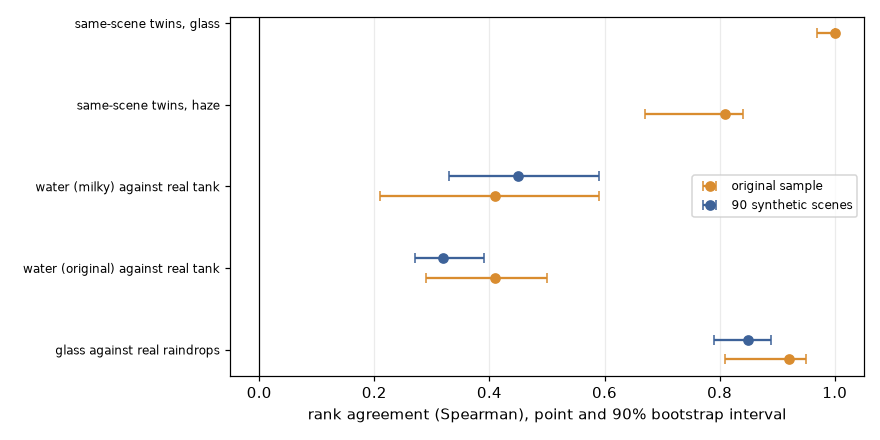
\includegraphics[width=.85\textwidth]{agreement_stability.png}\caption{\BOTH\ The same numbers as intervals.}\end{figure}
\begin{itemize}
\item \textbf{Glass is stable and strong:} +0.85 with 90 scenes (+0.79 to +0.89). The earlier 0.92 came from only 12 scenes; the true value is a little lower, still a strong agreement.
\item \textbf{Original synthetic water against the real tank is weak and stable:} about +0.3 (+0.27 to +0.39 with 90 scenes).
\item \textbf{Milky synthetic water is a modest improvement:} +0.45 (+0.33 to +0.59) against +0.32 for the original water. The intervals overlap a little, so the evidence is suggestive, not firm.
\item \textbf{The same-scene twins are the most reliable:} haze +0.81 (+0.67 to +0.84), glass +1.00. Where the scene and haze strength match, the synthetic model ranks the methods like the real picture does; the agreement fades when the scenes differ.
\end{itemize}

\subsection{So what can we trust?}
\begin{center}\small\begin{tabular}{p{4.2cm}p{11.3cm}}\toprule
Question & Verdict\\\midrule
Haze: best method & Real and calibrated synthetic agree that DCP alone is weak and a contrast step helps.\\
Haze: full ranking & Moderate to weak: +0.30 (calibrated) to +0.57 (original) on 90 indoor scenes, +0.09 on outdoor scenes with RESIDE's haze, +0.81 on the \emph{same scenes} as the real photos. Different scenes, and even different haze models, move it a lot.\\
Glass (raindrops) & Synthetic is a good stand-in: +0.85 (+0.79 to +0.89) on 90 scenes, up to +1.00 on the same scenes.\\
Water & \textbf{Partly checked.} The original (open-sea style) synthetic water disagrees with real tank pairs (+0.3 to +0.4, and a different winner). Milky synthetic water agrees on the verdict (nothing helps much, DCP hurts) but only modestly on the ranking (+0.4). On real ocean photos colour methods look best by eye. Ink: no real data.\\
Plastic & \textbf{Unchecked}: no real data exists. Treat as model results.\\
Original presets & Misleading for DCP on haze and stretch on glass; kept only for comparison.\\\bottomrule
\end{tabular}\end{center}

%--------------------------------------------------------------------
\section{Global or local? Where in the picture should a method act?}\label{sec:local}
Haze thickens with distance, raindrops cover only parts, plastic is the same everywhere. So should a method decide once for the whole picture (\emph{global}) or separately for each part (\emph{local})? We ran the same method both ways:
\begin{itemize}
\item \textbf{tiles:} cut the picture into a 2$\times$2, 4$\times$4 or 8$\times$8 grid, run the method on each tile, blend the tiles back smoothly;
\item \textbf{regions found from the picture} (\texttt{dark3}, \texttt{sharp2}): group pixels into three levels of ``haze thickness'' (from the dark channel) or into blurred and sharp areas, and run the method once per group;
\item \textbf{regions from the true depth} (\texttt{depth3}): only possible on \SYN\ pictures, so it shows the best a perfect region-finder could give.
\end{itemize}
\begin{figure}[H]\centering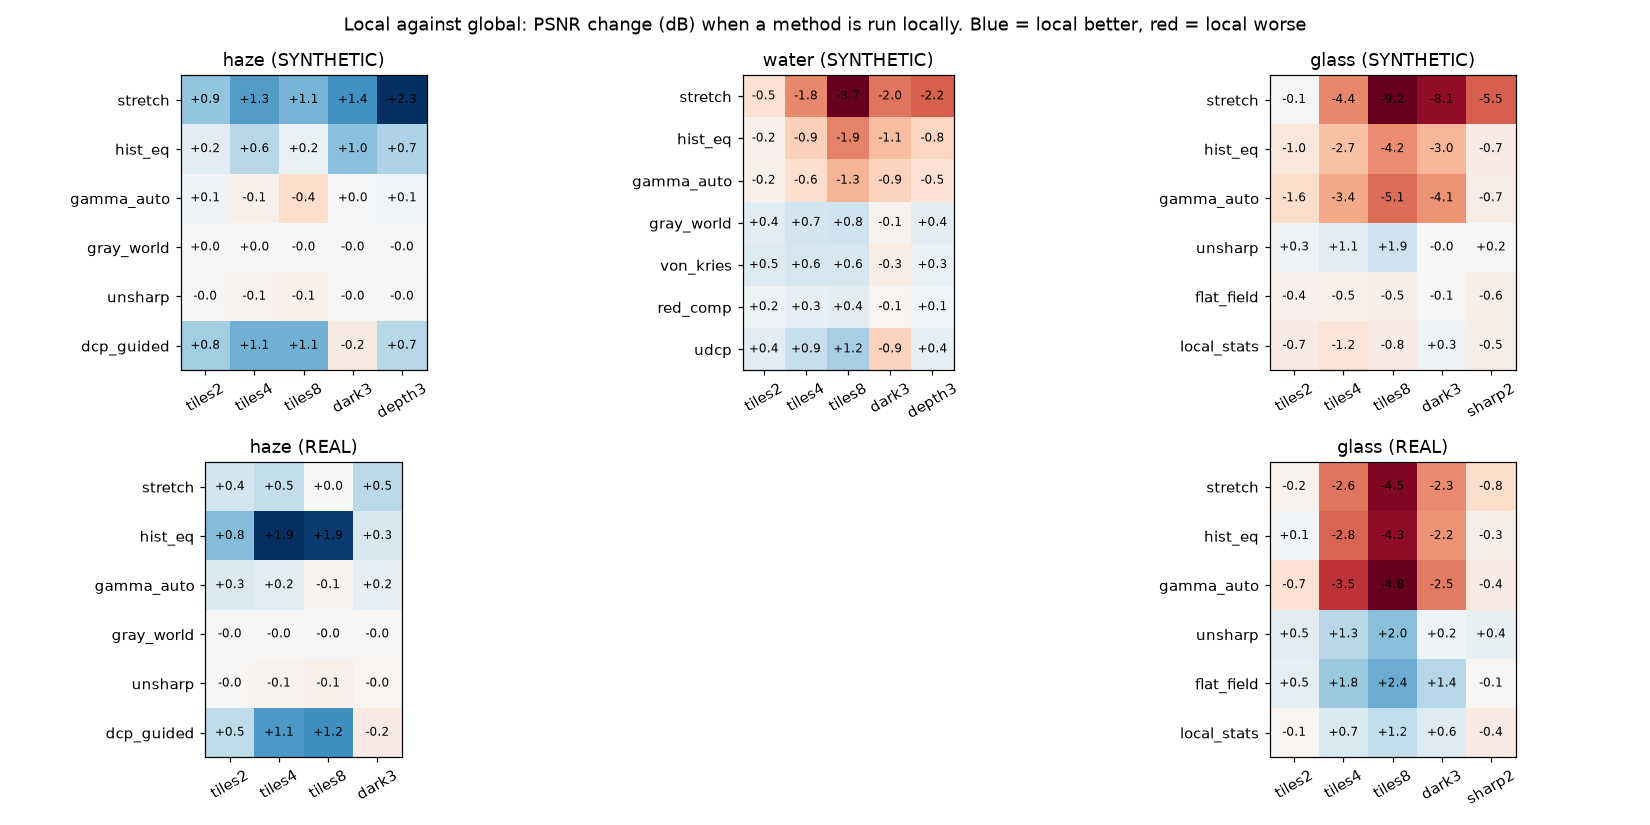
\includegraphics[width=\textwidth]{local_vs_global.png}\caption{\BOTH\ Change in PSNR (dB) when a method runs locally instead of globally. Blue: local is better; red: worse. Top row \SYN, bottom row \REAL. Water has no real pairs.}\end{figure}
\paragraph{What we see.}
\begin{itemize}
\item \textbf{Haze (local helps, on both kinds of pictures).} On real haze, histogram equalisation on 4$\times$4 tiles gains +1.95 dB (better on every picture) and turns a method that was worse than doing nothing (10.8 against 11.6 dB) into a useful one (12.7). Guided DCP gains +1.2 dB on 8$\times$8 tiles. On synthetic haze, stretch gains +2.3 dB when given the true depth regions. Depth is the useful information: it is what makes the haze differ from place to place.
\item \textbf{Water (small gains, synthetic only).} Colour methods gain a little locally (gray-world +0.8, von Kries +0.6), contrast methods lose.
\item \textbf{Glass (local hurts).} Stretch and histogram equalisation lose up to 9 dB when run per tile, on synthetic and real raindrops. A tile that contains a drop is stretched differently from its neighbour, which creates patchwork. The apparent gains of unsharp, flat-field and local-statistics are \emph{not} locality: these methods measure their scale as a share of the picture size, so on a small tile they act more weakly and drift towards doing nothing, which still beats every variant (24.5 dB on real).
\end{itemize}
\subsection{How many tiles?}
We repeated the comparison with every grid from 2$\times$2 to 12$\times$12 tiles. A grid with $n$ tiles per side cuts the picture into $n\times n$ tiles (4$\times$4 is 16 tiles).
\begin{figure}[H]\centering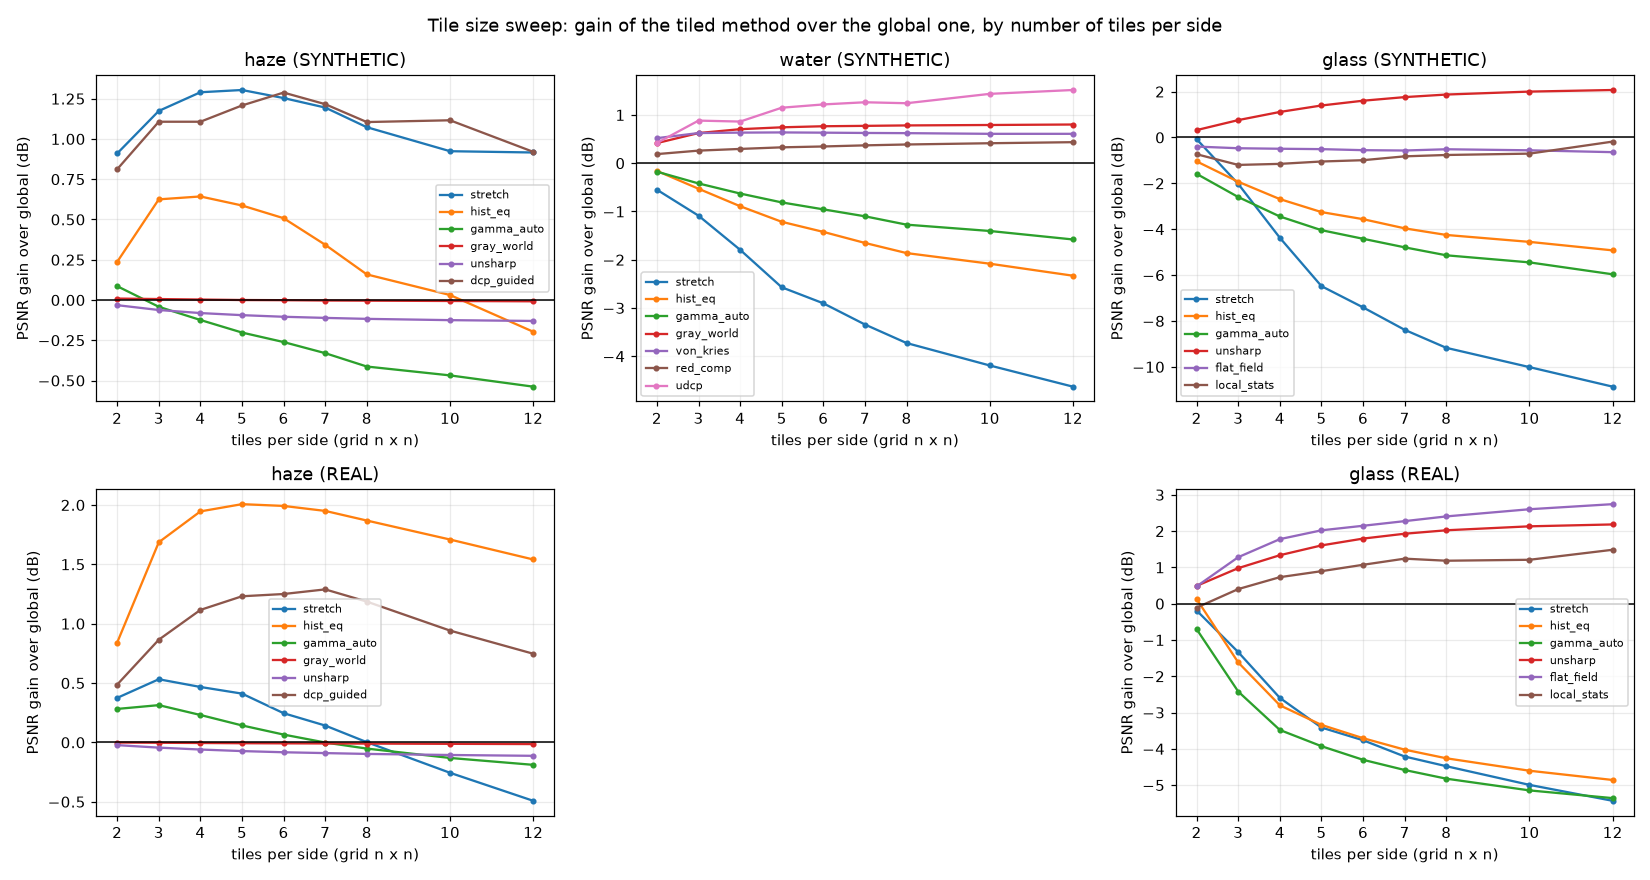
\includegraphics[width=\textwidth]{local_tile_sweep.png}\caption{\BOTH\ Gain over the global method for each grid size, one line per method. Top row \SYN, bottom row \REAL.}\end{figure}
\begin{table}[H]\centering\small
\begin{tabular}{llrrrrrrrrr}\toprule
Pictures & Medium & 2 & 3 & 4 & 5 & 6 & 7 & 8 & 10 & 12\\\midrule
\REAL & haze & +0.33 & +0.56 & \textbf{+0.62} & \textbf{+0.62} & +0.58 & +0.55 & +0.48 & +0.36 & +0.25\\
\SYN & haze & +0.34 & +0.47 & +0.47 & +0.47 & +0.45 & +0.39 & +0.30 & +0.25 & +0.16\\
\SYN & water & \textbf{+0.09} & +0.05 & $-$0.12 & $-$0.25 & $-$0.33 & $-$0.44 & $-$0.55 & $-$0.63 & $-$0.74\\
\REAL & glass & \textbf{+0.02} & $-$0.45 & $-$0.84 & $-$1.03 & $-$1.13 & $-$1.23 & $-$1.32 & $-$1.47 & $-$1.54\\
\SYN & glass & \textbf{$-$0.59} & $-$1.24 & $-$1.84 & $-$2.32 & $-$2.56 & $-$2.80 & $-$2.99 & $-$3.21 & $-$3.42\\\bottomrule
\end{tabular}
\caption{Mean PSNR gain (dB) over the global method, averaged over the methods tried per medium, by tiles per side. Best grid in bold.}\end{table}
\begin{itemize}
\item \textbf{Haze: about 4$\times$4 to 6$\times$6 is best, then the gain falls.} By method: histogram equalisation peaks at 5$\times$5 on real haze (+2.0, but the curve is flat from 4 to 8); DCP peaks later, at 6$\times$6 or 7$\times$7 (+1.3), because its own patch size is measured relative to the tile; gray-world and unsharp do not change.
\item \textbf{The best size is not the same across media.} In water the colour methods (gray-world, red compensation, UDCP) keep gaining up to 12$\times$12, while stretch and histogram equalisation lose more with every extra tile. In glass the less tiling the better: stretch falls from $-$0.1 dB at 2$\times$2 to $-$10.9 dB at 12$\times$12 on synthetic raindrops.
\item \textbf{Why:} haze changes smoothly with distance, so medium-sized tiles each see roughly constant haze but still enough picture to decide sensibly. Small tiles see too little content. Raindrops are patches, and a tile that contains one is stretched differently from its neighbour.
\end{itemize}
Unsharp, flat-field and local-statistics seem to improve on glass with more tiles. That is not locality: on a small tile they act more weakly and drift towards doing nothing.

\paragraph{Caution.} Findings come from one set of regions (three levels of dark channel) and a few tile sizes; PSNR penalises local re-stretching that shifts brightness; and the table of best local variants in the log is a maximum over several tries, so it is optimistic (the figure shows every try).

%--------------------------------------------------------------------
\section{Why does it work this way?}\label{sec:why}
\subsection{How long should a chain be? A mathematical check, then a test}
\label{sec:chainlength}
We searched chains of up to 3 steps. Would 4 or 5 steps help? Before searching, we asked what the mathematics allows.

\textbf{What the equations say.} Haze, water, a film on glass and plastic each damage a picture by (optionally) a blur and then a per-colour \emph{affine} map, $I=tJ+A(1-t)$. Affine maps compose into one affine map, so a single step (a stretch, a white balance) undoes any number of such layers, and the blur needs one more step. The damage is therefore invertible in \emph{one or two steps}. Two further facts give ceilings:
\begin{itemize}
\item \textbf{A ceiling for chains of whole-picture brightness steps.} Stretch, gamma, histogram equalisation, white balance and log are all a function of the pixel value, so a chain of any number of them is still one such function per colour. The best possible function (the \emph{oracle LUT}: for each input value, the average true value of the pixels that have it) is a ceiling for every such chain, however long.
\item \textbf{A ceiling for any chain on invertible damage.} Inverting with the true $t$ and $A$ is exact except for the rounding of the saved picture to 8 bits (a grey level of $1/255$), which the inversion multiplies by $1/t$. Its predicted PSNR is $-10\log_{10}\!\big(\overline{1/t^{2}}/(12\cdot255^{2})\big)$.
\end{itemize}
\begin{table}[H]\centering\scriptsize\tablein{chain_limits}\caption{\label{tab:chain_limits}\SYN\ Held-out PSNR (18 pictures): doing nothing; the best chain of 1, 2 and 3 steps (chosen on other pictures); the two ceilings; and the predicted PSNR of the true inverse. No inverse exists for raindrops.}\end{table}
\begin{figure}[H]\centering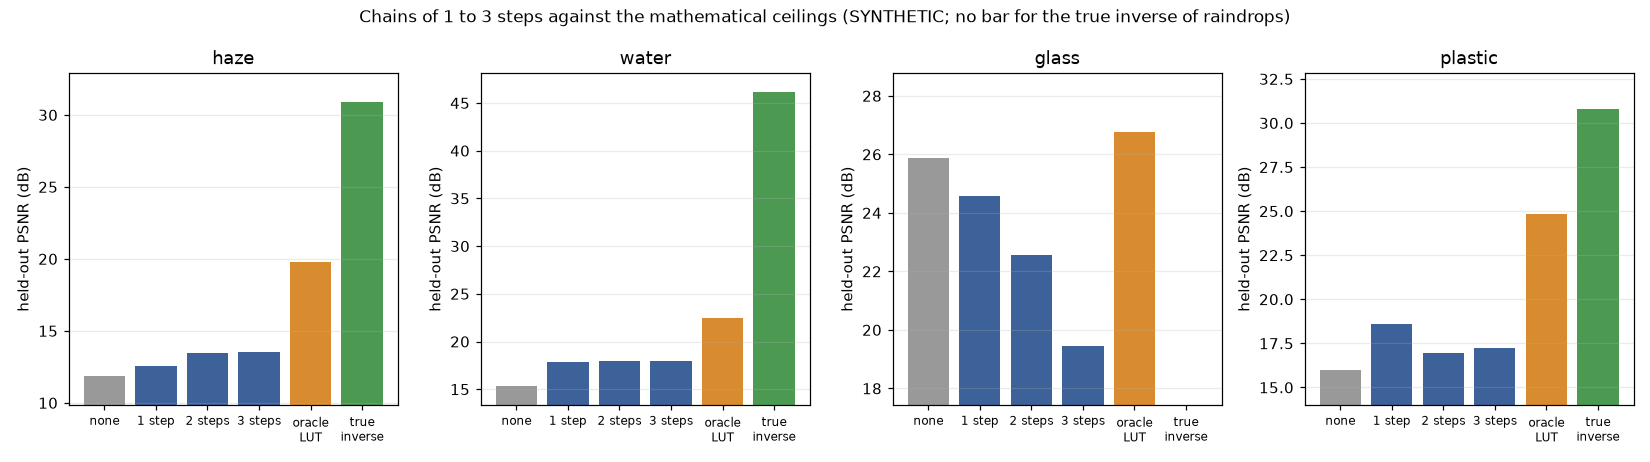
\includegraphics[width=.95\textwidth]{chain_limits.png}\caption{\SYN\ The best chains against the ceilings.}\end{figure}
\textbf{What we checked.}
\begin{itemize}
\item \textbf{The formula holds where the damage is affine.} Water: predicted 45.9 dB, measured 46.1 dB. For haze the measured value is higher than predicted (30.9 against 18.7) because the formula ignores that pictures are clipped to the valid range, so the error cannot grow without limit. For plastic the formula predicts 54 dB but the measured inverse is 30.8 dB: the missing 24 dB is the cost of undoing the blur, which the formula does not include.
\item \textbf{No chain reaches the ceilings, and the gap is large} (haze 13.5 against 30.9 dB for the true inverse; water 18.0 against 46.1; plastic 17.2 against 30.8). The limit is not the number of steps, it is that the chain must \emph{guess} $t$, $A$, the tint and the blur from the damaged picture alone. Even the best single affine map (which needs the clear picture) is far above the found chains for plastic (24.4 against 17.2 dB).
\item \textbf{So extra steps should add nothing once the damage is undone.} The prediction: the gain of a step beyond the 2nd or 3rd is zero within noise.
\end{itemize}
\textbf{The test.} We searched chains of 1 to 3 steps completely and chains of 4 and 5 steps by extending the best 40 chains of the previous length (a beam search), choosing the best chain of each length on one set of scenes (A). A second set (B) chose the length (the shortest within one standard error of the best), and a third set (C, 36 pictures, never used to choose anything) reports the result.
\begin{table}[H]\centering\scriptsize\tablein{longer_chains}\caption{\SYN\ Held-out PSNR of the best chain of each length (0 = doing nothing). B chose the length; C was never used.}\end{table}
\begin{figure}[H]\centering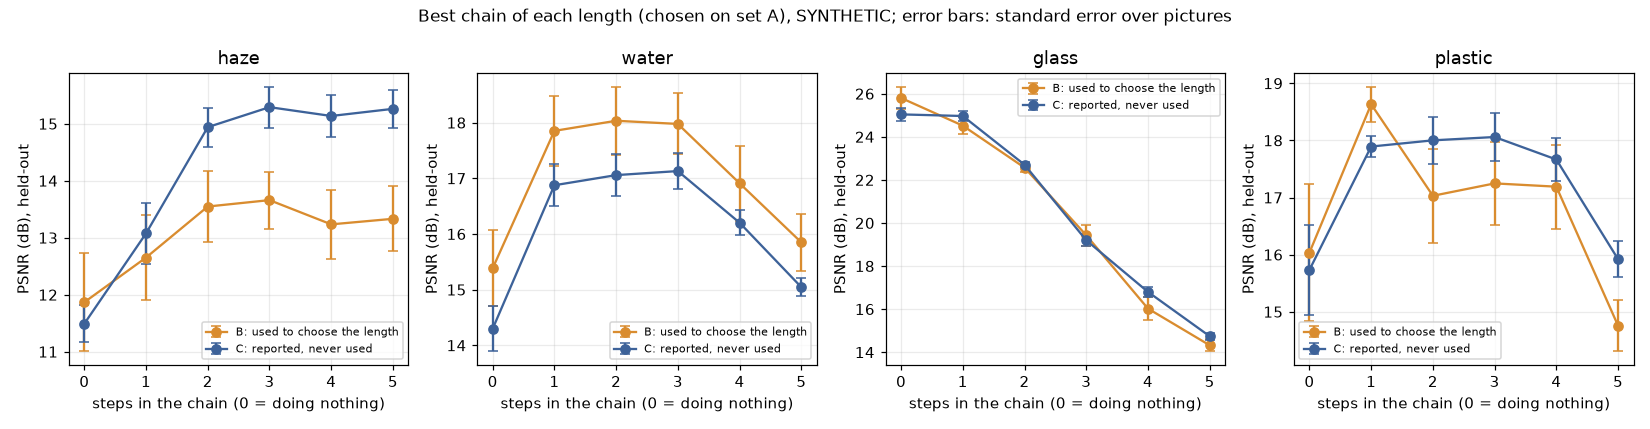
\includegraphics[width=.95\textwidth]{longer_chains.png}\caption{\SYN\ Best chain of each length against the number of steps. Error bars: standard error over pictures.}\end{figure}
\begin{itemize}
\item \textbf{The prediction held.} The gain of the 4th step is $-0.15\pm0.06$ dB (haze), $-0.9\pm0.2$ (water), $-2.4\pm0.2$ (glass), $-0.4\pm0.1$ (plastic) on set C, and the 5th step gains $+0.13\pm0.13$ at best (haze) and loses 1 to 2 dB elsewhere. Among the chains searched, those of 4 and 5 steps were not even best on the search set.
\item \textbf{Where the curve peaks.} Haze: 2 to 3 steps (set C: 3 steps +0.35$\pm$0.14 over 2; set B, with half the pictures, chose 2). Water: 2 steps. Plastic: 1 to 3 steps are tied within noise. Glass: every step lowers the score, and no chain beats doing nothing.
\item \textbf{More steps usually hurt.} Each added step is another estimate with its own error, and the errors add up: the best five-step water chain scored 15.0 dB on set C, 1.8 dB below the best one-step chain (16.9 dB) and only 0.7 dB above doing nothing (14.3 dB).
\end{itemize}
\textbf{The same test on real pictures \REAL.} Real haze (from the 185 pairs: sets of 24, 23 and 46 pairs) and real tank water (TUB; sets of 31, 30 and 59 pairs), with the same pool of steps and the same design.
\begin{table}[H]\centering\scriptsize\tablein{longer_chains_real}\caption{\REAL\ Held-out PSNR of the best chain of each length (0 = doing nothing). B chose the length; C was never used.}\end{table}
\begin{figure}[H]\centering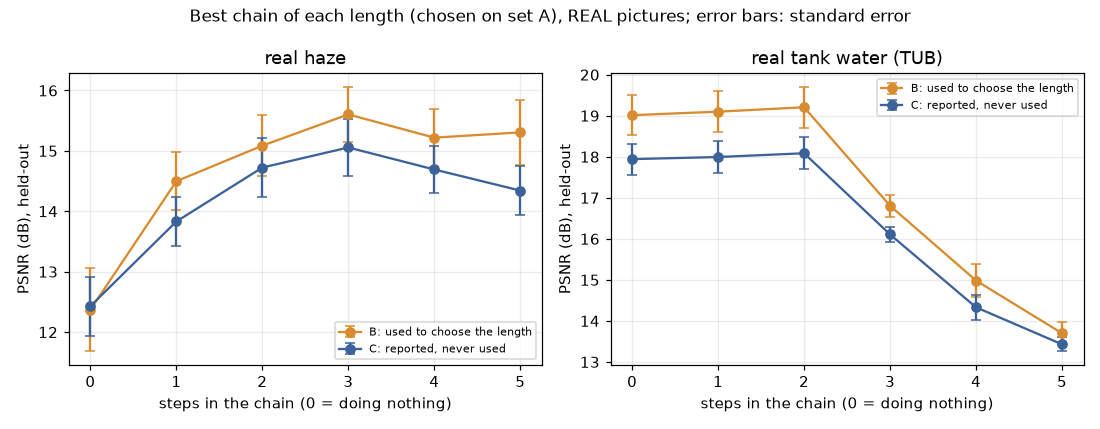
\includegraphics[width=.8\textwidth]{longer_chains_real.png}\caption{\REAL\ Best chain of each length. Error bars: standard error over pictures.}\end{figure}
\begin{itemize}
\item \textbf{Real haze peaks at 3 steps and then stops.} Going from 2 to 3 steps still gains $+0.52\pm0.17$ dB (B) and $+0.33\pm0.08$ (C); the 4th step gains $-0.38\pm0.39$ and $-0.36\pm0.27$, the 5th $+0.09\pm0.14$ and $-0.35\pm0.08$. The best 3-step chain is \texttt{dcp\_guided > gray\_world > clahe} (white balance between the haze removal and the contrast step). That a third step still pays is not a contradiction of the 1-to-2-step theory: real haze is tinted, which our model does not include, and the gray-world step undoes that tint.
\item \textbf{Real tank water: 2 steps are as far as it goes, and the gain is tiny.} \texttt{red\_comp > unsharp} gains $0.2$ dB over doing nothing (19.2 against 19.0 dB on B). The 3rd step loses $2.4\pm0.3$ dB, the 4th $1.8\pm0.3$, the 5th $1.3\pm0.3$: three or more steps are worse than doing nothing.
\end{itemize}
The prediction held on real pictures too: chains of 4 and 5 steps do not help. The useful range is up to 3 steps for real haze and 2 for real tank water.

Conclusion: chains of 2 to 3 steps are the useful range, on synthetic and on real pictures; the damage is invertible in one to two steps and the remaining headroom comes from estimating the parameters better, not from adding steps.

\subsection{Haze removal by subtraction}
Haze adds a smooth glow. Could we simply estimate that glow and subtract it? A \emph{constant} glow does not work (11.4 dB, worse than doing nothing at 12.2). A \emph{local} glow that follows the depth, estimated from how much the detail has faded, reaches \textbf{15.0 dB on real haze} (guided DCP: 13.9; the best possible simple frequency filter: 15.4, an upper bound). The lesson: the veil depends on distance, so it must be estimated locally. One caution: the settings of this method came from the same four datasets, so it needs testing on other scenes.
\begin{table}[H]\centering\scriptsize\tablein{frequency_subtraction}\caption{Haze removal by subtraction on the held-out real pairs (``real'', \REAL) and on their synthetic twins (``twin'', \SYN).}\end{table}

\subsection{Subtraction combined with the other tools}
Subtraction was first tried alone. We then put both subtraction methods into the pool with the DCP family and the contrast tools, and tried every chain of up to three different steps (9 steps, 585 chains), choosing the best on one set of pictures and judging it on another. For real haze we used only the half of each dataset that was \emph{not} used to measure the method's two priors, so the test is not contaminated. (An earlier run that mixed the halves made the subtraction method look 0.7 dB better, so we threw it away.)
\begin{figure}[H]\centering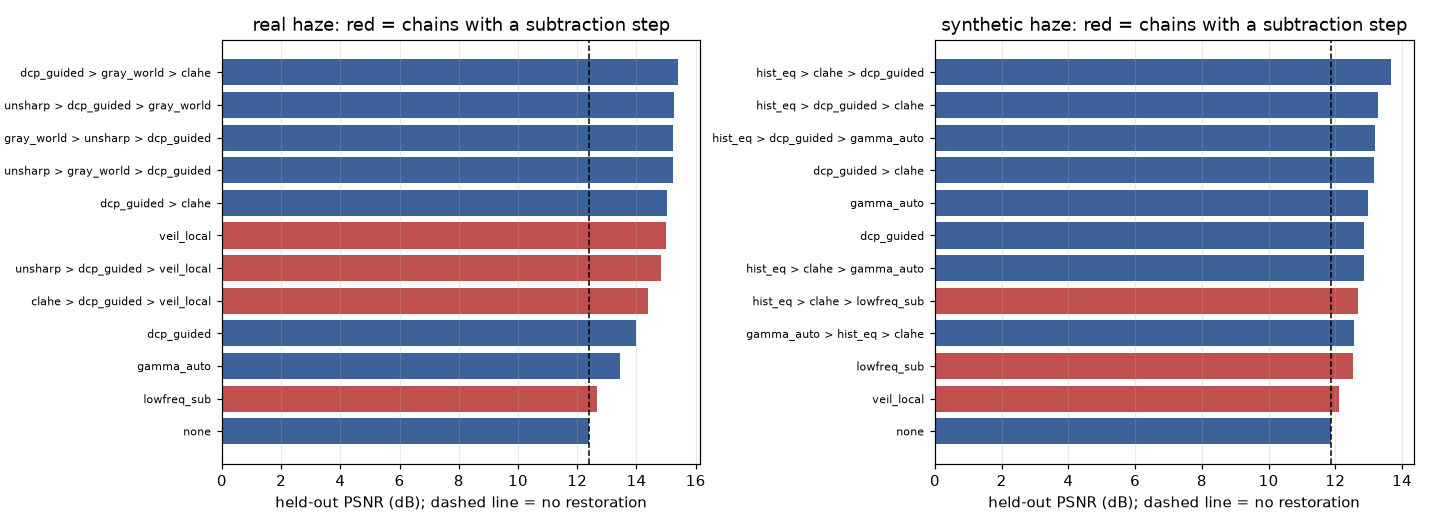
\includegraphics[width=.95\textwidth]{subtraction_combos.png}\caption{Held-out PSNR of the best chains and some references (dashed line: no restoration). Red bars contain a subtraction step. Left: \REAL\ haze (23 pairs); right: \SYN\ calibrated haze (18 pictures).}\end{figure}
\begin{itemize}
\item \textbf{On real haze, subtraction alone is as good as anything:} 14.98 dB, tied with DCP then CLAHE (15.02). The best chain overall, \texttt{unsharp > gray\_world > dcp\_guided} (15.24), does not use it, and the best chain that does use it is slightly lower (14.84). So \emph{no combination with subtraction beat the best combination without it}.
\item \textbf{Where in the chain it goes matters.} Averaged over all chains, a subtraction step placed \emph{last} helps (13.7 dB for three-step chains), placed \emph{first} does not (12.4, the same as chains without it). Subtraction inverts the haze equation, so it works best on a picture that has not been altered; filters applied before it break the equation it assumes.
\item \textbf{On synthetic haze the order of the winners reverses:} DCP-based chains win (13.66) and subtraction chains lose (12.67). This is the same real-versus-synthetic disagreement as before, now for a method family.
\item One chain (\texttt{blind\_veil\_local > tarel > dcp\_guided}) produces invalid pictures and was dropped.
\end{itemize}

\subsection{Why DCP fails on water}
DCP guesses the glow from the brightest pixels. In water the true glow is a dark blue-green (about 0.34) but bright objects fool DCP into guessing 0.84. An error of 0.50 in $A$ spoils every pixel. Colour methods avoid this because they need no glow estimate.
\begin{figure}[H]\centering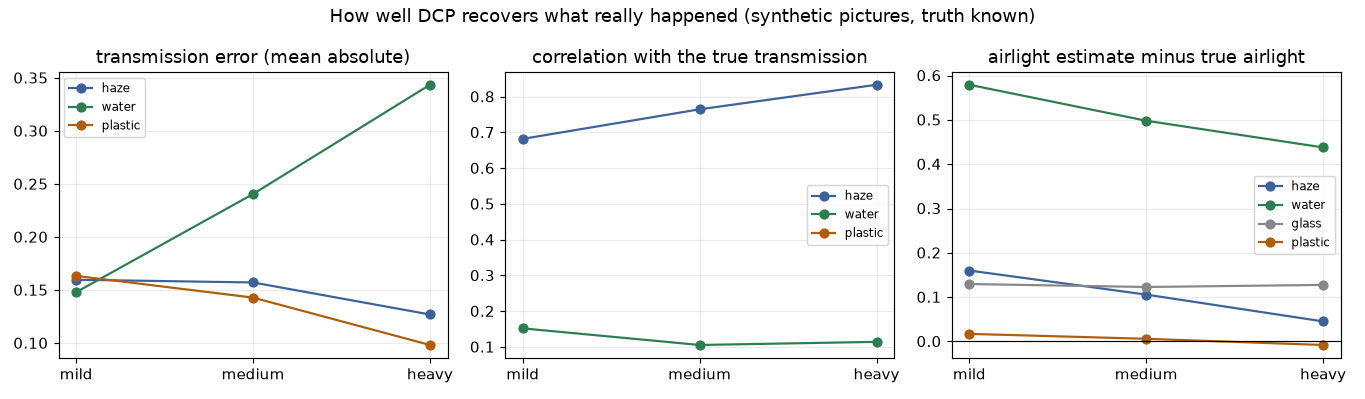
\includegraphics[width=.9\textwidth]{failure_transmission.png}\caption{\SYN\ How well DCP finds the transmission $t$ for haze, water and plastic (correlation with the truth: +0.76 haze, +0.11 water).}\end{figure}

%--------------------------------------------------------------------
\section{How good can a repair be? Equations, refinements and limits}
\label{sec:limits}
This section sets our equations beside the ones in the literature, asks what the real pictures say should be added, writes the inverse of every function we use, and explains why the measured scores sit far below the best possible.

\subsection{General equations and ours}
Entries marked $^\dagger$ are quoted from memory of the papers and should be checked before they are cited.
{\small\begin{longtable}{p{1.3cm}p{8.3cm}p{5.8cm}}
\toprule Medium & Common equation in the literature & Ours\\\midrule\endhead
Air & Atmospheric scattering model (Koschmieder; McCartney; Narasimhan and Nayar): $I=Jt+A(1-t)$, $t=e^{-\beta d}$. Variants: a $\beta_c$ per colour, a $\beta(x)$ that varies over the picture, a glow $A(x)$ for night scenes, a forward-scatter blur. & The same equation, with one scalar $\beta$ and one scalar glow $A$.\\
Water & Jaffe--McGlamery: total light = direct + forward scatter + backscatter, where forward scatter is the direct signal blurred. Simplified form (Chiang and Chen): $I_c=J_ce^{-\beta_cd}+B_c(1-e^{-\beta_cd})$.$^\dagger$ Revised (Akkaynak and Treibitz): the direct and the backscatter coefficients differ, $\beta^D\ne\beta^B$.$^\dagger$ & The simplified form with a $\beta_c$ per colour. No forward scatter, and $\beta^D=\beta^B$.\\
Plastic & ASTM D1003 haze: diffuse light (scattered by more than 2.5$^\circ$) as a share of the total transmitted light. Imaging models: a point-spread function with a narrow core and a wide halo, plus attenuation and veil. & A Gaussian blur, a tint and a milky veil. No wide halo, no scratches.\\
Glass & Raindrops (Qian et al.): $I=(1-M)\odot B+R$, a mask blend.$^\dagger$ Dirt (Eigen et al.): an opacity-weighted dirt layer.$^\dagger$ Veiling glare: stray light $I=J+g\,(K\!*\!J)$ with a wide kernel $K$; Stiles--Holladay $L=10E/\theta^2$.$^\dagger$ & A film as haze with a depth-free $t$, smudges as a blur blend, droplets as a blend with a blurred scene. Real drops refract an inverted miniature of the scene, which a blur only imitates.\\\bottomrule
\end{longtable}}

\subsection{What the real pictures say to add}
For every real pair we fitted four nested models of how the clear picture became the degraded one, and scored how well each reproduces the real degraded picture (PSNR of the fitted picture; higher means the model explains the real picture better).
\begin{table}[H]\centering\scriptsize\resizebox{\textwidth}{!}{\tablein{model_refinement}}\caption{\REAL\ Fit of nested models to the real pairs. ``One $t$ and $A$'': $I=aJ+b$. ``Per colour'': a separate $a_c,b_c$ per channel. ``+ blur'': the scene is blurred first (best width per pair). ``+ local maps'': a separate map in each cell of a 4$\times$4 grid (96 parameters per pair, so part of this gain is flexibility). $t$ and $A$ are the means of the per-colour fit.}\end{table}
\begin{itemize}
\item \textbf{Haze: the biggest missing piece is that $t$ varies across the picture} (+8.2 dB), which means depth. Colour dependence adds +1.3 dB: blue is attenuated most ($t=0.34,0.30,0.26$ for red, green, blue) and the glow is bluish ($A=0.61,0.63,0.69$; our first model used 0.92 for all colours). Blur adds only +0.2 dB.
\item \textbf{Milky tank water: the colour is in the glow, not in the attenuation.} The glow is yellow-brown ($A=0.57,0.53,0.42$) while $t$ is nearly the same for all colours (0.30, 0.29, 0.27), which is the opposite of the open-sea model. Per colour +3.5 dB, blur +1.2 dB (width 2.8\% of the picture), uneven light over the picture +7.0 dB (the lamp).
\item \textbf{Raindrops: none of the affine refinements explains them} (26.1 to 27.0 dB). They need a patch model with refraction.
\end{itemize}
We then built the refined haze (per-colour $\beta$ and glow, plus the blur, fitted with the values above and calibrated to the real severity as before) and tested, as in Test 7, whether it ranks the methods like real haze does.
\begin{table}[H]\centering\scriptsize\tablein{outdoor_haze}\caption{\SYN\ Rank agreement of five synthetic hazes with the 185 real haze pairs (17 methods), and the winners.}\end{table}
\begin{itemize}
\item \textbf{The refinements did not improve the ranking} (+0.28, against +0.30 for the first calibrated haze and +0.57 for the original haze). Their picture statistics are no closer either (signature distance 0.35, 0.27, 0.42 against 0.34, 0.23, 0.17).
\item \textbf{A uniform fog is the worst} ($-$0.12): its damage is one global affine map, so a plain stretch undoes it almost exactly (47.7 dB), which is not what happens on real haze. This confirms that the dependence on depth matters.
\item So the missing ingredient for matching the ranking is not colour or blur. We have not found it: the original haze, which looks least like the real fog in its statistics, ranks the methods closest to real haze.
\end{itemize}

\subsection{The inverse of every function we use}
Every limit is also limited by the rounding of the saved picture to 8 bits, which each division by $t$ multiplies: PSNR $\le -10\log_{10}\!\big(\overline{1/t^2}/(12\cdot255^2)\big)$.
{\small\begin{longtable}{p{2.5cm}p{6.1cm}p{6.8cm}}
\toprule Function & Inverse it computes & Theoretical limit\\\midrule\endhead
\texttt{stretch} & $J=(I-b)/a$, exact for one global affine map & Fails where $t$ varies across the picture.\\
\texttt{gamma}, \texttt{log}, \texttt{hist\_eq}, \texttt{hist\_spec}, \texttt{eq\_hsi} & The inverse of a monotone map applied to the pixel values (equalisation needs the clear picture's histogram) & Ceiling: the best possible map per colour, the \emph{oracle LUT}.\\
\texttt{gray\_world}, \texttt{white\_patch}, \texttt{von\_kries} & $J_c=I_c/g_c$ & Ignores the glow offset and relies on a scene assumption.\\
\texttt{red\_comp} & A heuristic, $R'=R+(\bar G-\bar R)(1-R)G$; the true inverse is $R=R_{\mathrm{obs}}e^{\beta_Rd}$, which needs the depth & Restores only the mean of red.\\
\texttt{dcp}, \texttt{dcp\_guided} & $J=\dfrac{I-A}{\max(t,t_0)}+A$, with $t=1-\omega\,\mathrm{dark}(I/A)$ & Exact if $t$ and $A$ are right. With $t_0=0.1$ noise is amplified up to 10$\times$ (a cap of about 39 dB).\\
\texttt{udcp} & The same, with the dark channel from green and blue & Needs red already lost.\\
\texttt{tarel} & $J=(I-V)/(1-V)$ & Assumes a white glow.\\
\texttt{blind\_veil} & $J=(I-\hat V)/\hat t$ & Assumes the local clear brightness is near the prior mean.\\
\texttt{clahe} & A local monotone map; no unique inverse & Noise grows with the clip limit.\\
\texttt{unsharp} & $I+k(I-h\!*\!I)$, the first term of the series that inverts a blur & Amplifies high-frequency noise.\\
\texttt{wiener}, \texttt{cls}, \texttt{richardson\_lucy} & $\hat J=\dfrac{H^*}{|H|^2+K}\hat I$ for a Gaussian blur, $H=e^{-2\pi^2\sigma^2f^2}$ & Detail above $f^*\approx\sqrt{\ln\mathrm{SNR}/(2\pi^2\sigma^2)}$ is lost.\\
\texttt{flat\_field} & $J=I/s$ with $s$ a wide blur & Also removes true slow scene content.\\
\texttt{homomorphic} & Inverts $I=s\cdot r$ in the log domain & Needs the lighting to be purely low-frequency.\\
\texttt{fusion} & A weighted blend, not an inverse & The output stays between its inputs.\\\bottomrule
\end{longtable}}
For the Wiener limit, rounding noise of 0.0011 and a signal of 0.2 give $f^*\approx0.51/\sigma$ (an estimate): our plastic blur ($\sigma\approx1.5$ pixels) is nearly invertible up to 0.34 cycles per pixel, the heaviest ($\sigma\approx3$) only up to 0.17.

\textbf{How the limits combine in a chain.} (1) A chain of pointwise steps is one monotone map per colour, so its ceiling is the oracle LUT however long it is. (2) Affine layers compose, $J=(I-b_{\mathrm{tot}})/a_{\mathrm{tot}}$ with $a_{\mathrm{tot}}=\prod t_i$ and $b_{\mathrm{tot}}=\sum_iA_i(1-t_i)\prod_{j>i}t_j$; the last layer is undone first. An affine map commutes with a normalised blur, so in an ideal world their order does not matter; in practice it does, because each step is an estimate and clipping to $[0,1]$ breaks the commutation.

\subsection{Why the measured scores are far below the best possible}
Table~\ref{tab:chain_limits} (Section~\ref{sec:chainlength}) shows chains at 13 to 18 dB against true inverses at 30 to 46 dB. The gap has four parts, which we separate by giving the method more and more of the truth.
\begin{itemize}
\item \textbf{The per-pixel transmission.} A whole-picture step cannot know that far pixels are hazier. At medium severity the haze chain reaches 13.4 dB and the best global affine map (which uses the clear picture) 14.9, the best global map of any shape (the LUT) 19.7, and the true per-pixel inverse 33.2 dB. The step from the LUT to the true inverse (+13.5 dB for haze, +26 dB for water) is the cost of $t(x)$.
\item \textbf{Estimating the glow.} The table below gives DCP the truth piece by piece on synthetic haze. With the true glow, DCP rises from 12.9 to 15.0 dB. With the true $t$ but the \emph{estimated} glow, the result is 10.8 dB, worse than DCP itself: an error $\Delta A$ in the glow becomes an error $\Delta A/t$ in the picture.
\item \textbf{Estimating $t$.} With the true glow, DCP's own $t$ gives 15.0 dB and the true $t$ gives 22.3 dB (with the floor $t_0$): the dark-channel guess of $t$ costs 7.3 dB.
\item \textbf{Rounding and the blur.} At heavy haze the true inverse itself is poor (14.3 dB, below the 18.2 dB of the oracle LUT), because $t$ is tiny and the 8-bit rounding is multiplied by $1/t$. For plastic, inverting the blur costs about 5 dB (oracle affine 23.9 and true inverse 29.1 at medium).
\end{itemize}
\begin{table}[H]\centering\scriptsize\resizebox{\textwidth}{!}{\tablein{gap_haze}}\caption{\SYN\ DCP given the truth piece by piece (calibrated synthetic haze, 18 held-out pictures; PSNR in dB).}\end{table}
\textbf{Are any results almost the best possible?} Yes, in two situations. At \emph{heavy haze} the chain reaches 12.4 dB against a true inverse of only 14.3 dB, and in 5 of the 18 pictures the best chain is within 3 dB of the true inverse. For \emph{raindrops} the best chains are within 1 dB of the oracle LUT in 10 of 18 pictures, but that ceiling is only 0.9 dB above doing nothing, so there is nothing to gain. For haze and water at mild and medium severity no chain comes within 1 dB of the LUT.

\subsection{Why the gaps are so large, and which pictures are beyond repair}
\label{sec:beyond}
Six things separate a measured score from the theoretical one, roughly from the most to the least important.
\begin{enumerate}
\item \textbf{The theory is told the truth; the method is not.} The true inverse uses the true $t(x)$ for every pixel, the true glow and the true blur. A method must guess them from the damaged picture alone. For $t(x)$ this is an ill-posed problem (a bright grey patch may be a hazy far wall or a near white wall), so even a good guess is wrong in places, and a wrong $t$ or $A$ is magnified by $1/t$.
\item \textbf{The priors fail on some pictures.} DCP assumes a dark pixel in every patch (the clear pictures have a mean dark channel of 0.12 to 0.21, not 0), a stretch assumes the clear picture spans the full range, white balance assumes a grey scene.
\item \textbf{The information may be gone.} Rounding to 8 bits (and sensor noise in real pictures) is multiplied by $1/t$; where $t$ is small the signal is buried. This is the only case where no method, however clever, can succeed.
\item \textbf{The model is wrong for real pictures.} Real haze has a coloured glow and varies over the picture; real raindrops replace patches (Section~\ref{sec:limits}).
\item \textbf{PSNR punishes brightness and colour shifts} that look acceptable, so an equally good-looking restoration scores lower.
\item \textbf{The functions and their settings may be incomplete}: the plastic result of Section~\ref{sec:theorychains} (+8 dB from a per-colour stretch and the true blur width).
\end{enumerate}
\paragraph{Beyond repair.} We call a synthetic picture \emph{beyond repair} when more than half of its pixels have $t<0.0055$: there the rounding error of 0.0011, multiplied by $1/t$, exceeds a typical scene contrast of 0.2, so the signal-to-noise ratio is below one and not even the exact inverse can bring the pixel back. For real pictures $t$ is unknown, so we use what is left of the scene's detail (the sharpness ratio: the detail of the degraded picture relative to the clear one) and ask whether any method we tried restores the structure (SSIM) and not just the brightness.
\begin{table}[H]\centering\scriptsize\resizebox{\textwidth}{!}{\tablein{beyond_repair_synthetic}}\caption{\SYN\ Classes of the 18 held-out pictures per medium and severity. ``Near the theory'' means the best chain is within 3 dB of the true inverse, or above it (heavy haze, where the true inverse itself fails).}\end{table}
\begin{itemize}
\item \textbf{Haze, mild and medium, and water at every severity, are estimation-limited:} all 18 pictures in each row have a true inverse 10 dB or more above the best chain. Nothing is lost; the methods simply cannot see $t(x)$. (Our synthetic water never loses pixels, since its largest attenuation, $e^{-4.8}=0.008$, stays above the limit.)
\item \textbf{Heavy synthetic haze contains pictures beyond repair:} on average 46\% of the pixels are unrecoverable; 6 of the 18 pictures are beyond repair, and for 11 more the best chain already matches or beats the (failing) inverse.
\end{itemize}
\begin{table}[H]\centering\scriptsize\tablein{beyond_repair_real}\caption{\REAL\ What the best of the methods tried can do, by how much detail is left (sharpness ratio). Real haze: 185 pairs; real tank water: 120 pairs.}\end{table}
\begin{figure}[H]\centering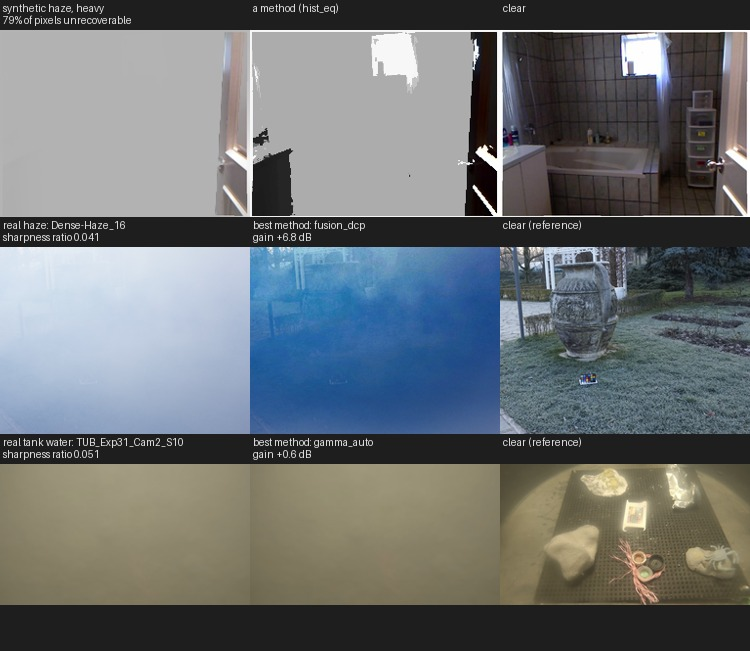
\includegraphics[width=.85\textwidth]{beyond_repair.jpg}\caption{Pictures beyond repair. Row 1: \SYN\ heavy haze, 79\% of the pixels unrecoverable (histogram equalisation shows flat grey where the information is gone). Row 2: \REAL\ Dense-Haze, the lowest detail left (sharpness ratio 0.04); the best method (fusion after DCP) gains 6.8 dB, but the result is a blue wash in which the vase is not back. Row 3: \REAL\ tank water at the highest turbidity: a white-out; the best method gains 0.6 dB and recovers nothing.}\end{figure}
\begin{itemize}
\item \textbf{Real Dense-Haze: 38 of its 55 pairs are close to beyond repair.} The sharpness ratio is below 0.1 for all 38. Their PSNR still improves by 4.7 dB, but SSIM only rises from 0.30 to 0.46, against 0.65 to 0.80 for the lighter hazes: brightness and colour are restored, the structure only in part. The other three datasets (O-HAZE, I-HAZE, NH-Haze) have no pair below 0.1.
\item \textbf{Real tank water: no picture is repaired.} The best of 17 methods gains about 0.5 dB on average (0.2 to 0.7 dB across turbidity bands), SSIM stays at 0.665 to 0.670 for the densest 39 pairs (the white-outs), and 54 to 86\% of the pairs gain less than 0.5 dB in each detail band. At low turbidity there is little to repair (the unrepaired picture already scores 21 dB); at high turbidity the detail is gone.
\item \textbf{Raindrops} are a different case: the covered patches are gone, but the rest of the picture is fine, so the picture is not beyond repair but beyond \emph{global} repair; a method that detects and fills drops (inpainting) is outside this study.
\end{itemize}

\subsection{The best chain against the theoretical restoration, in pictures}
\label{sec:theorypics}
For every synthetic held-out picture we took the best of all chains tried (the earlier searches and the chains derived from the inverse in the next subsection; chosen with the answer known, so slightly optimistic) and compared it with the theoretical restoration: the true inverse, or for raindrops (which have no inverse) the best possible map of pixel values, the oracle LUT. The three rows of each figure are the case with the smallest gap, a typical (median) gap and the largest gap. Columns: degraded, best chain, oracle LUT, theoretical restoration, clear.
\begin{figure}[H]\centering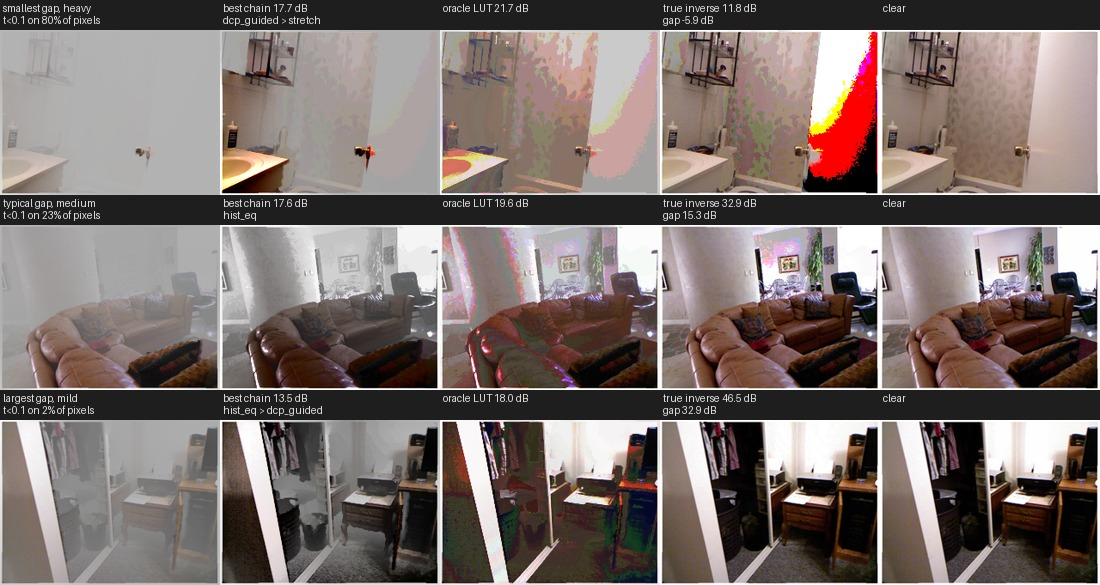
\includegraphics[width=\textwidth]{theory_haze.jpg}\caption{\SYN\ Haze. Top: heavy haze, where the best chain beats the true inverse. Middle: medium haze. Bottom: mild haze, the largest gap.}\end{figure}
\begin{itemize}
\item \textbf{Smallest gap, heavy haze: the chain beats the theory ($-5.9$ dB).} Here $t<0.1$ on 80\% of the pixels, so the 8-bit rounding of the picture is multiplied by $1/t$ (up to $10^8$ in $1/t^2$) and the true inverse breaks down (saturated white and red patches). A chain that raises contrast without dividing by $t$ is better.
\item \textbf{Typical gap, medium haze (15 dB).} The true inverse is almost exact (32.9 dB); the chain (histogram equalisation, 17.6 dB) brightens the whole picture but cannot know that the far wall is hazier than the near sofa, so a veil remains where $t$ is small.
\item \textbf{Largest gap, mild haze (33 dB).} Only 2\% of the pixels have $t<0.1$, so the true inverse is nearly perfect (46.5 dB), but any chain that cannot see $t(x)$ leaves the depth gradient (the grey wash at the back of the room) and cannot restore the colours.
\end{itemize}
\begin{figure}[H]\centering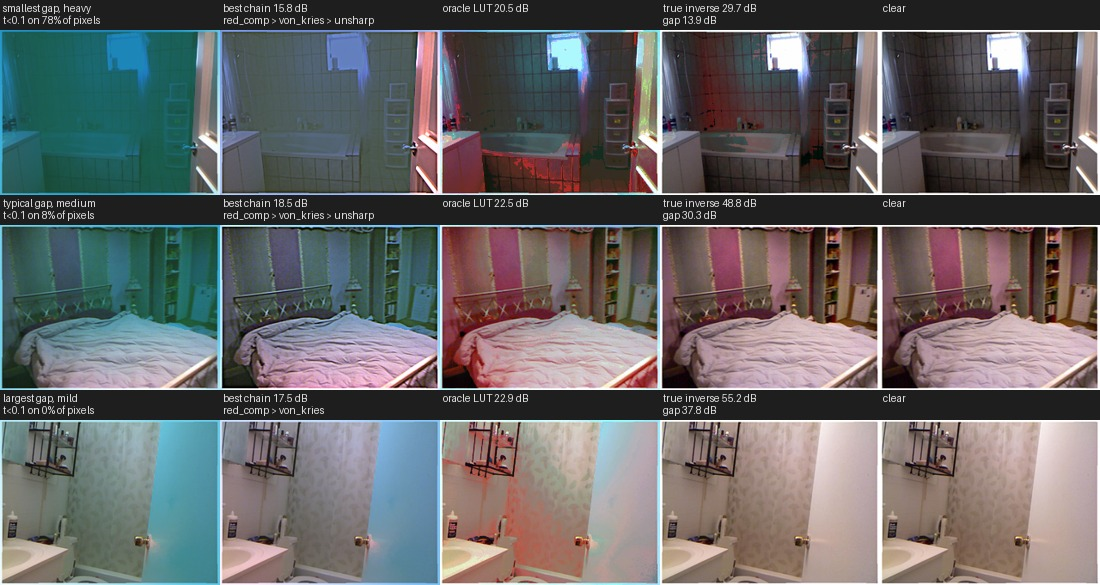
\includegraphics[width=\textwidth]{theory_water.jpg}\caption{\SYN\ Open-sea style water, same layout.}\end{figure}
Water behaves like haze: the gap is small only when rounding limits the inverse (heavy: $t<0.1$ on 78\% of the pixels, true inverse 29.7 dB, gap 14 dB), and grows to 30 to 38 dB at medium and mild severity where the inverse is almost exact (49 to 55 dB) but the chain's colour correction is global (17.5 to 18.5 dB).
\begin{figure}[H]\centering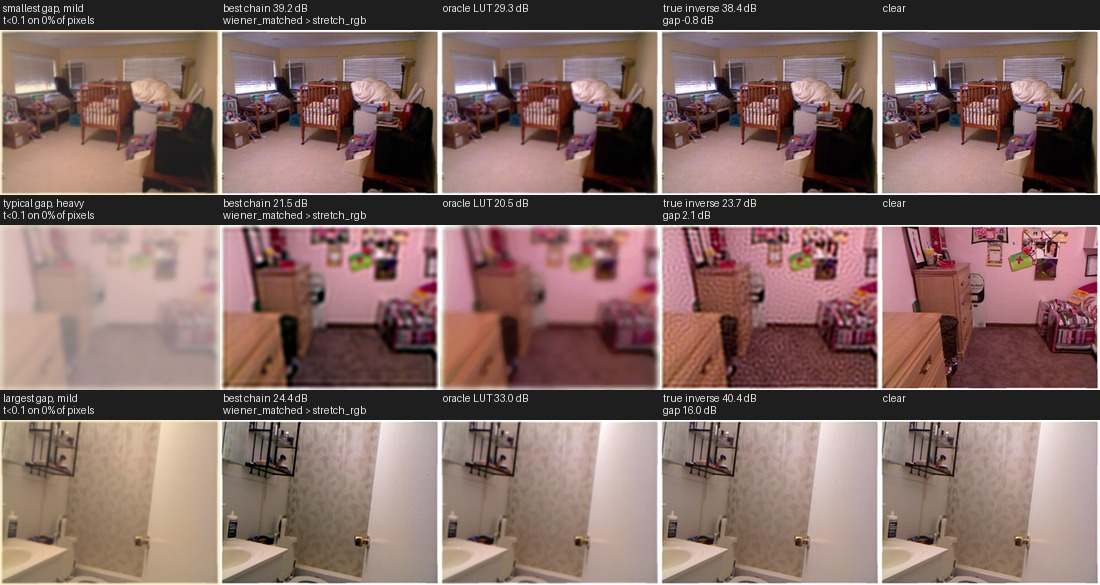
\includegraphics[width=\textwidth]{theory_plastic.jpg}\caption{\SYN\ Plastic. The best chain is the derived \texttt{wiener\_matched > stretch\_rgb} in all three cases.}\end{figure}
\begin{itemize}
\item \textbf{Smallest gap, mild plastic ($-0.8$ dB):} the chain is essentially the inverse (undo the blur, then one per-colour range), and it matches the true inverse (39.2 against 38.4 dB).
\item \textbf{Typical gap, heavy plastic (2.1 dB):} a 3-pixel blur; the Wiener filter cannot recover detail above about 0.17 cycles per pixel (Section~\ref{sec:limits}), so the result stays softer than the true inverse.
\item \textbf{Largest gap, mild plastic (16 dB):} the blur is easy, but the per-colour stretch \emph{assumes the clear picture spans the full range from black to white}. This bathroom is bright with few deep shadows, so the likely cause (not tested) is that the stretch maps the wrong range and leaves a brightness and colour offset; the true inverse knows the true gain and offset.
\end{itemize}
\begin{figure}[H]\centering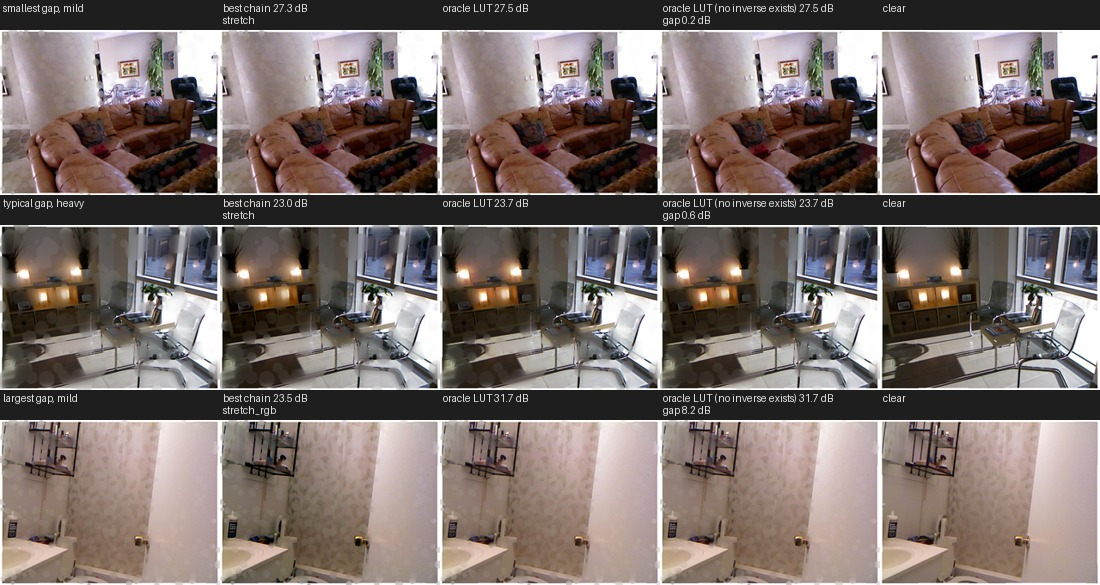
\includegraphics[width=\textwidth]{theory_glass.jpg}\caption{\SYN\ Raindrops. The theoretical column is the oracle LUT (no inverse exists).}\end{figure}
For raindrops the typical and smallest gaps are only 0.2 to 0.6 dB: the best chain (a plain stretch) is already close to the best possible whole-picture map, and that map is only about 1 dB above doing nothing. The largest gap (8 dB) is a picture where the oracle map, which sees the answer, does much better than any rule that has to guess; we did not look into why.

\subsection{Chains derived from the inverse equations, and whether we had tried them}
\label{sec:theorychains}
The inverse of each medium is a short list of operations (undo the gain and offset per colour; undo the depth-dependent transmission; undo the blur), and each operation has a function that approximates it. We built the chains in the order the inverse asks for and tested them next to the best chains of the earlier searches. One function was missing: the stretch in the earlier searches used a single range for all colours, so it could not undo a different gain and offset per colour. We added \texttt{stretch\_rgb} (a separate range per colour), and a Wiener filter whose blur width equals the true blur of the severity (\texttt{wiener\_matched}).
{\small\begin{longtable}{llllrr}
\toprule
pictures & chain & origin & tried before? & PSNR & vs best earlier chain \\
\midrule
\endhead
synthetic haze & none & -- & -- & 11.61 & -3.22 $\pm$ 0.374 \\
synthetic haze & dcp\_guided $>$ stretch & derived from the inverse & no & 12.94 & -1.89 $\pm$ 0.326 \\
synthetic haze & gray\_world $>$ dcp\_guided & derived from the inverse & yes & 12.95 & -1.89 $\pm$ 0.313 \\
synthetic haze & gray\_world $>$ dcp\_guided $>$ stretch & derived from the inverse & no & 12.83 & -2.00 $\pm$ 0.312 \\
synthetic haze & dcp\_guided $>$ gray\_world & derived from the inverse & yes & 12.98 & -1.85 $\pm$ 0.324 \\
synthetic haze & dcp\_guided $>$ gray\_world $>$ stretch\_rgb & derived from the inverse & no & 12.89 & -1.94 $\pm$ 0.314 \\
synthetic haze & tarel $>$ stretch & derived from the inverse & no & 10.92 & -3.91 $\pm$ 0.309 \\
synthetic haze & blind\_veil\_local $>$ stretch & derived from the inverse & no & 12.16 & -2.68 $\pm$ 0.346 \\
synthetic haze & stretch\_rgb $>$ dcp\_guided & derived from the inverse & no & 12.29 & -2.55 $\pm$ 0.303 \\
synthetic haze & dcp\_guided $>$ gamma\_auto & derived from the inverse & yes & 13.54 & -1.29 $\pm$ 0.307 \\
synthetic haze & hist\_eq & earlier search & -- & 13.07 & -1.76 $\pm$ 0.325 \\
synthetic haze & hist\_eq $>$ dcp\_guided & earlier search & -- & 14.54 & -0.30 $\pm$ 0.123 \\
synthetic haze & hist\_eq $>$ clahe $>$ dcp\_guided & earlier search & -- & 14.83 & +0.00 $\pm$ 0.0 \\
synthetic haze & ceilings: oracle LUT / true inverse &  &  & 19.4 / 30.0 &  \\
synthetic water & none & -- & -- & 14.64 & -2.76 $\pm$ 0.131 \\
synthetic water & stretch\_rgb & derived from the inverse & no & 14.82 & -2.58 $\pm$ 0.194 \\
synthetic water & gray\_world $>$ stretch\_rgb & derived from the inverse & no & 15.32 & -2.08 $\pm$ 0.19 \\
synthetic water & red\_comp $>$ stretch\_rgb & derived from the inverse & no & 15.85 & -1.55 $\pm$ 0.192 \\
synthetic water & stretch\_rgb $>$ von\_kries & derived from the inverse & no & 16.81 & -0.59 $\pm$ 0.157 \\
synthetic water & udcp $>$ stretch\_rgb & derived from the inverse & no & 11.74 & -5.66 $\pm$ 0.2 \\
synthetic water & red\_comp $>$ von\_kries $>$ stretch\_rgb & derived from the inverse & no & 16.73 & -0.67 $\pm$ 0.175 \\
synthetic water & von\_kries $>$ stretch\_rgb & derived from the inverse & no & 16.38 & -1.01 $\pm$ 0.168 \\
synthetic water & von\_kries & earlier search & -- & 17.17 & -0.23 $\pm$ 0.058 \\
synthetic water & red\_comp $>$ von\_kries & earlier search & -- & 17.35 & -0.05 $\pm$ 0.052 \\
synthetic water & red\_comp $>$ von\_kries $>$ unsharp & earlier search & -- & 17.40 & +0.00 $\pm$ 0.0 \\
synthetic water & ceilings: oracle LUT / true inverse &  &  & 21.2 / 45.5 &  \\
synthetic plastic & none & -- & -- & 15.81 & -2.33 $\pm$ 0.559 \\
synthetic plastic & stretch $>$ wiener & derived from the inverse & no & 20.26 & +2.12 $\pm$ 0.293 \\
synthetic plastic & wiener $>$ stretch & derived from the inverse & no & 20.41 & +2.28 $\pm$ 0.225 \\
synthetic plastic & stretch\_rgb $>$ wiener & derived from the inverse & no & 21.99 & +3.85 $\pm$ 0.372 \\
synthetic plastic & wiener $>$ stretch\_rgb & derived from the inverse & no & 21.73 & +3.60 $\pm$ 0.313 \\
synthetic plastic & stretch\_rgb $>$ richardson\_lucy & derived from the inverse & no & 22.17 & +4.04 $\pm$ 0.326 \\
synthetic plastic & stretch\_rgb $>$ wiener\_matched & derived from the inverse & no & 26.01 & +7.87 $\pm$ 0.768 \\
synthetic plastic & wiener\_matched $>$ stretch\_rgb & derived from the inverse & no & 26.57 & +8.43 $\pm$ 0.803 \\
synthetic plastic & clahe & earlier search & -- & 18.14 & +0.00 $\pm$ 0.0 \\
synthetic plastic & wiener $>$ dcp\_guided & earlier search & -- & 17.68 & -0.45 $\pm$ 0.358 \\
synthetic plastic & wiener $>$ unsharp $>$ dcp\_guided & earlier search & -- & 17.76 & -0.38 $\pm$ 0.369 \\
synthetic plastic & ceilings: oracle LUT / true inverse &  &  & 24.2 / -- &  \\
synthetic glass & none & -- & -- & 25.36 & +0.50 $\pm$ 0.24 \\
synthetic glass & flat\_field $>$ stretch & derived from the inverse & yes & 19.58 & -5.28 $\pm$ 0.292 \\
synthetic glass & stretch $>$ flat\_field & derived from the inverse & yes & 19.59 & -5.27 $\pm$ 0.294 \\
synthetic glass & flat\_field $>$ stretch\_rgb & derived from the inverse & no & 19.55 & -5.31 $\pm$ 0.29 \\
synthetic glass & stretch\_rgb & derived from the inverse & no & 24.67 & -0.19 $\pm$ 0.03 \\
synthetic glass & stretch & earlier search & -- & 24.86 & +0.00 $\pm$ 0.0 \\
synthetic glass & stretch $>$ unsharp & earlier search & -- & 22.64 & -2.22 $\pm$ 0.169 \\
synthetic glass & flat\_field $>$ unsharp $>$ stretch & earlier search & -- & 19.28 & -5.58 $\pm$ 0.326 \\
synthetic glass & ceilings: oracle LUT / true inverse &  &  & 26.2 / -- &  \\
real haze & none & -- & -- & 12.41 & -2.83 $\pm$ 0.38 \\
real haze & dcp\_guided $>$ stretch & derived from the inverse & no & 12.70 & -2.54 $\pm$ 0.248 \\
real haze & gray\_world $>$ dcp\_guided & derived from the inverse & yes & 14.29 & -0.95 $\pm$ 0.254 \\
real haze & gray\_world $>$ dcp\_guided $>$ stretch & derived from the inverse & no & 13.08 & -2.15 $\pm$ 0.221 \\
real haze & dcp\_guided $>$ gray\_world & derived from the inverse & yes & 14.39 & -0.85 $\pm$ 0.246 \\
real haze & dcp\_guided $>$ gray\_world $>$ stretch\_rgb & derived from the inverse & no & 13.30 & -1.94 $\pm$ 0.191 \\
real haze & tarel $>$ stretch & derived from the inverse & no & 9.81 & -5.43 $\pm$ 0.34 \\
real haze & blind\_veil\_local $>$ stretch & derived from the inverse & no & 13.82 & -1.42 $\pm$ 0.348 \\
real haze & stretch\_rgb $>$ dcp\_guided & derived from the inverse & no & 13.47 & -1.76 $\pm$ 0.177 \\
real haze & dcp\_guided $>$ gamma\_auto & derived from the inverse & yes & 13.24 & -2.00 $\pm$ 0.317 \\
real haze & dcp\_guided $>$ gray\_world $>$ clahe & earlier search & -- & 15.24 & +0.00 $\pm$ 0.0 \\
real haze & dcp\_guided $>$ clahe & earlier search & -- & 14.85 & -0.39 $\pm$ 0.076 \\
real water & none & -- & -- & 18.30 & -0.16 $\pm$ 0.017 \\
real water & stretch\_rgb & derived from the inverse & no & 12.86 & -5.60 $\pm$ 0.273 \\
real water & gray\_world $>$ stretch\_rgb & derived from the inverse & no & 12.86 & -5.60 $\pm$ 0.273 \\
real water & red\_comp $>$ stretch\_rgb & derived from the inverse & no & 12.85 & -5.61 $\pm$ 0.273 \\
real water & stretch\_rgb $>$ von\_kries & derived from the inverse & no & 12.61 & -5.86 $\pm$ 0.277 \\
real water & udcp $>$ stretch\_rgb & derived from the inverse & no & 11.79 & -6.67 $\pm$ 0.37 \\
real water & red\_comp $>$ von\_kries $>$ stretch\_rgb & derived from the inverse & no & 12.85 & -5.61 $\pm$ 0.273 \\
real water & von\_kries $>$ stretch\_rgb & derived from the inverse & no & 12.86 & -5.60 $\pm$ 0.273 \\
real water & red\_comp $>$ unsharp & earlier search & -- & 18.46 & +0.00 $\pm$ 0.0 \\
real water & unsharp & earlier search & -- & 18.36 & -0.10 $\pm$ 0.006 \\
\bottomrule
\end{longtable}
}
\begin{itemize}
\item \textbf{Plastic: the derived chains win by a wide margin.} \texttt{wiener\_matched > stretch\_rgb} scores 26.6 dB against 18.1 for the best earlier chain (+8.4 dB), and even with the default blur width \texttt{stretch\_rgb > richardson\_lucy} reaches 22.2 dB (+4.0). The earlier search missed them for two reasons: its pool had no per-colour stretch, and its Wiener filter always assumed one blur width. This chain also lies above the oracle LUT (24.2 dB), as it must: the LUT bounds only chains of pointwise steps, and a deblur is not pointwise.
\item \textbf{Haze: the derived chains do not beat the earlier ones.} \texttt{dcp\_guided > gamma\_auto} (13.5 dB) and the others stay 1.3 to 3.9 dB below the best earlier chain (14.8 dB), and adding a stretch after DCP lowers the score on real haze (13.1 against 14.4 without it). On real haze the best derived chain, \texttt{dcp\_guided > gray\_world} (14.4), is 0.85 dB below the earlier \texttt{dcp\_guided > gray\_world > clahe}.
\item \textbf{Water: close, but not better.} \texttt{stretch\_rgb > von\_kries} reaches 16.8 dB on synthetic water, 0.6 dB below the best earlier chain; the per-colour stretch alone (14.8) is worse than white balance (17.2) because the damage varies with depth, which a global range cannot follow. On the real tank water the per-colour stretch is harmful (12.9 dB against 18.3 for doing nothing): the near-uniform milky picture has almost no range for the percentiles to estimate, so the stretch amplifies noise.
\item \textbf{Glass:} chains that assume a slow film (\texttt{flat\_field}) lower the score by 5 dB, as raindrops are not a film.
\item \textbf{Had we tried them?} Only some. Chains made of the earlier pool's functions at their default settings had been searched (marked ``yes''). Chains using \texttt{stretch}, \texttt{stretch\_rgb}, the matched Wiener filter or the subtraction methods inside a medium's own pool had not (marked ``no'').
\end{itemize}
\textbf{So should the functions, their settings and their order change?} Yes, where the theory says what the inverse needs: for plastic the settings (the blur width) and a per-colour stretch matter by 4 to 8 dB, more than any reordering. For haze and water the settings are near their optimum (previous subsection) and the derived chains do not beat the searched ones. The order of deblur and stretch commutes in theory; in practice deblurring first is 0.6 dB better (26.6 against 26.0), because the stretch percentiles are estimated on a blurred picture.

\subsection{Should the settings and the order of the steps change?}
We tuned the settings inside the best real-picture chains on one set of pictures and judged them on two others (the same disjoint sets as in Section~\ref{sec:chainlength}).
\begin{table}[H]\centering\scriptsize\tablein{tune_chain}\caption{\REAL\ Default against tuned settings of the best chains (A chose the settings; B and C are held out). Gain: mean $\pm$ standard error, dB.}\end{table}
\begin{itemize}
\item \textbf{Real haze, \texttt{dcp\_guided > gray\_world > clahe}:} tuning $\omega$, $t_0$, the patch size, the CLAHE clip and tile count gains $+0.06\pm0.25$ dB (B) and $+0.20\pm0.15$ (C), within the noise. The defaults are already near the best: the score surface is flat around them.
\item \textbf{Real tank water, \texttt{red\_comp > unsharp}:} stronger red compensation (2.0) and a wider unsharp mask ($\sigma=0.03$) gain $+0.48\pm0.09$ (B) and $+0.33\pm0.05$ (C), small but consistent. Both best values sit at the edge of the grid, so the best setting may be stronger still.
\item \textbf{The order matters more than the settings.} The order of the same steps changes the score by up to 3.1 dB (Stage 4d), a subtraction step placed last helps and placed first does not, while tuning the settings gains 0.1 to 0.5 dB. The theory agrees: undo the last layer first, and give each step an unmodified picture to estimate from.
\end{itemize}

\section{Conclusions and limits}
\begin{enumerate}
\item The one equation $I=tJ+A(1-t)$ explains all four media; the frequency view confirms it.
\item \textbf{DCP is the right tool only for haze,} and even there it is weak on real photos without a following contrast step.
\item \textbf{Something beats DCP:} on real haze, DCP then CLAHE (+0.9 dB over DCP alone on all 185 pairs) and local-glow subtraction (+1.2 dB over DCP on its held-out pairs); on synthetic water, colour correction (+5.0 dB over DCP). On real turbid tank water nothing beat doing nothing and DCP was far worse (11.5 against 18.7 dB); on real ocean photos colour correction looks best by eye. Synthetic water made milky (matching the tank) reproduces that verdict; a dark ink cloud, in contrast, is helped by brightening methods.
\item \textbf{Order matters,} by up to 3.1 dB, and an extra step can help or hurt.
\item \textbf{Made-up pictures help but need checking.} Our first presets gave misleading winners; calibrating to real pictures fixed glass fully and haze partly.
\item \textbf{Raindrops cannot be repaired by global methods,} and running methods per tile does not fix that. Nothing beat doing nothing.
\item \textbf{For haze, local is better than global:} running histogram equalisation or DCP tile by tile gained 1 to 2 dB on real haze, best at roughly 4$\times$4 to 6$\times$6 tiles; depth is the information that matters. The best tile size differs by medium (water: colour methods like many tiles; glass: none).
\item \textbf{Some pictures are beyond repair.} Where more than half of a synthetic picture has $t<0.0055$ (6 of 18 heavy-haze pictures), the information is gone; on real pictures the densest Dense-Haze (38 pairs) is repaired in brightness but only partly in structure, and the real tank water is not repaired at any turbidity.
\item \textbf{The best possible is far above what any chain reaches, and the gap is estimation, not steps.} The true inverse is 13 to 26 dB above the chains at medium severity; its parts are the per-pixel transmission (depth), the estimate of the glow (an error $\Delta A$ becomes $\Delta A/t$) and of $t$, rounding at heavy haze, and the blur for plastic. Real pictures also ask for per-colour glow and local variation, but refining the synthetic haze that way did not make it rank the methods more like real haze. Tuning the settings inside the best chains gains 0.1 to 0.5 dB; the order of the steps matters more.
\end{enumerate}
\textbf{Limits.} Plastic is unchecked against real pictures, and real water is only partly checked (a tank with milky turbidity and a nearly clear reference; ocean photos without a reference; ink has no real data at all). Own captures are still to come. The haze ranking mismatch across scenes is unexplained beyond the scene argument. The subtraction method's settings were fitted on the test data's source datasets.

\textbf{Reproducibility.} Everything is rerunnable stage by stage (\texttt{code/experiments/run\_stages.py}); a full run takes about 9 minutes on 16 CPU cores. All numbers in this report are read from \texttt{results/tables/}. Every finding and failed attempt is in \texttt{log.md}.

%--------------------------------------------------------------------
\appendix
\section{Does the frequency theory hold?}
\begin{table}[H]\centering\tiny\tablein{theory_checks}\caption{Predicted against measured detail retention (mid-band ratio). Error 0.0 means exact. ``haze\_depth'' is haze that changes with distance, where a plain formula was off (0.103) and a detail-weighted one fixed it (0.029). The raindrop formula improved from 0.176 to 0.097.}\end{table}
\begin{figure}[H]\centering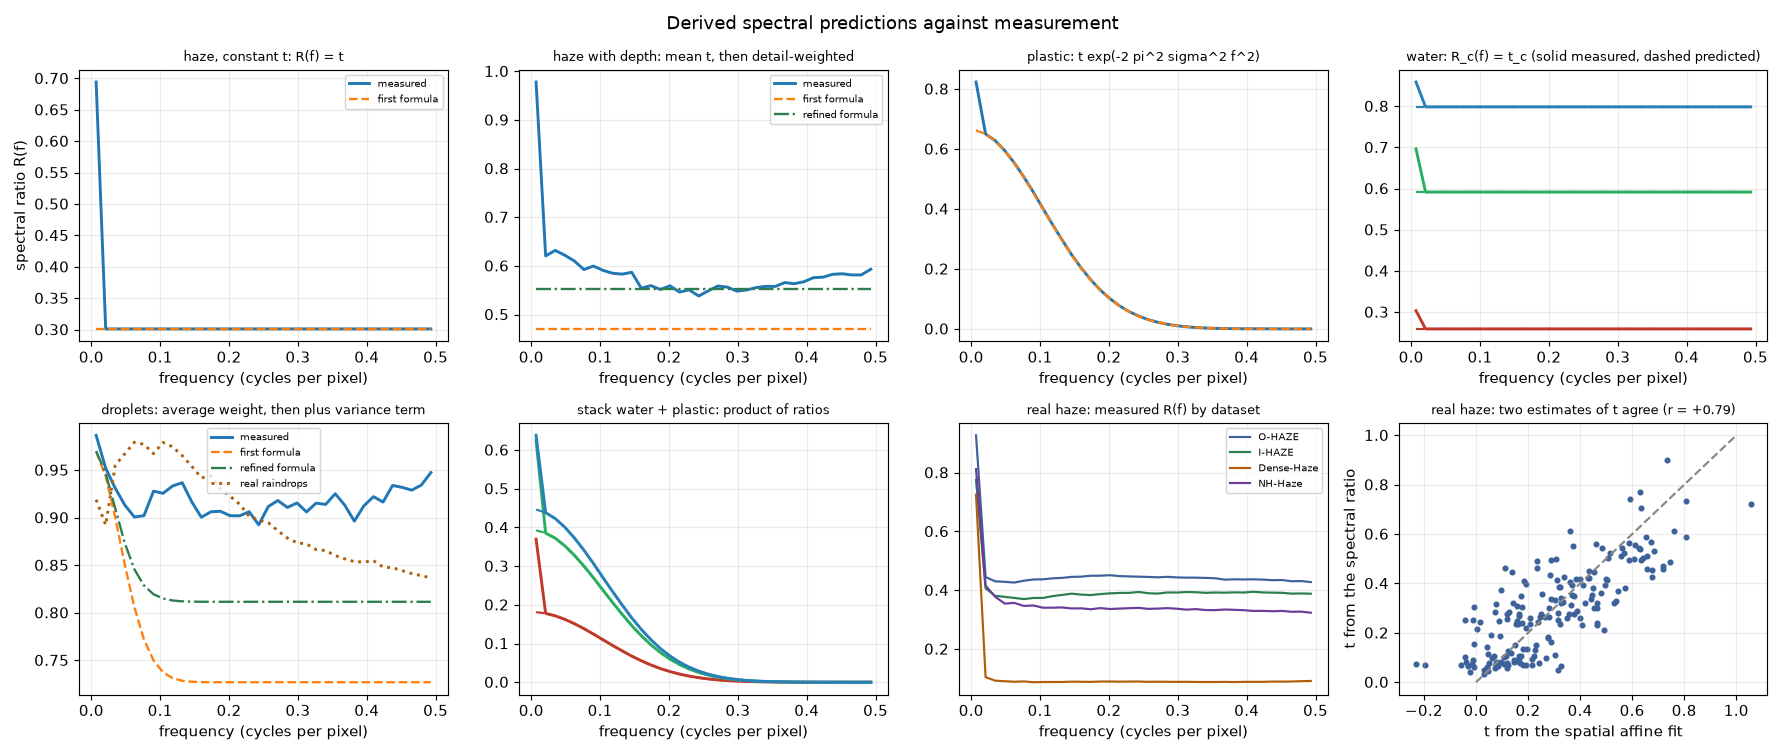
\includegraphics[width=.95\textwidth]{theory_spectral_ratio.png}\caption{\SYN\ Measured against predicted detail retention per medium (frequency on the horizontal axis).}\end{figure}

\section{Parameter and severity sweeps \SYN}
\begin{figure}[H]\centering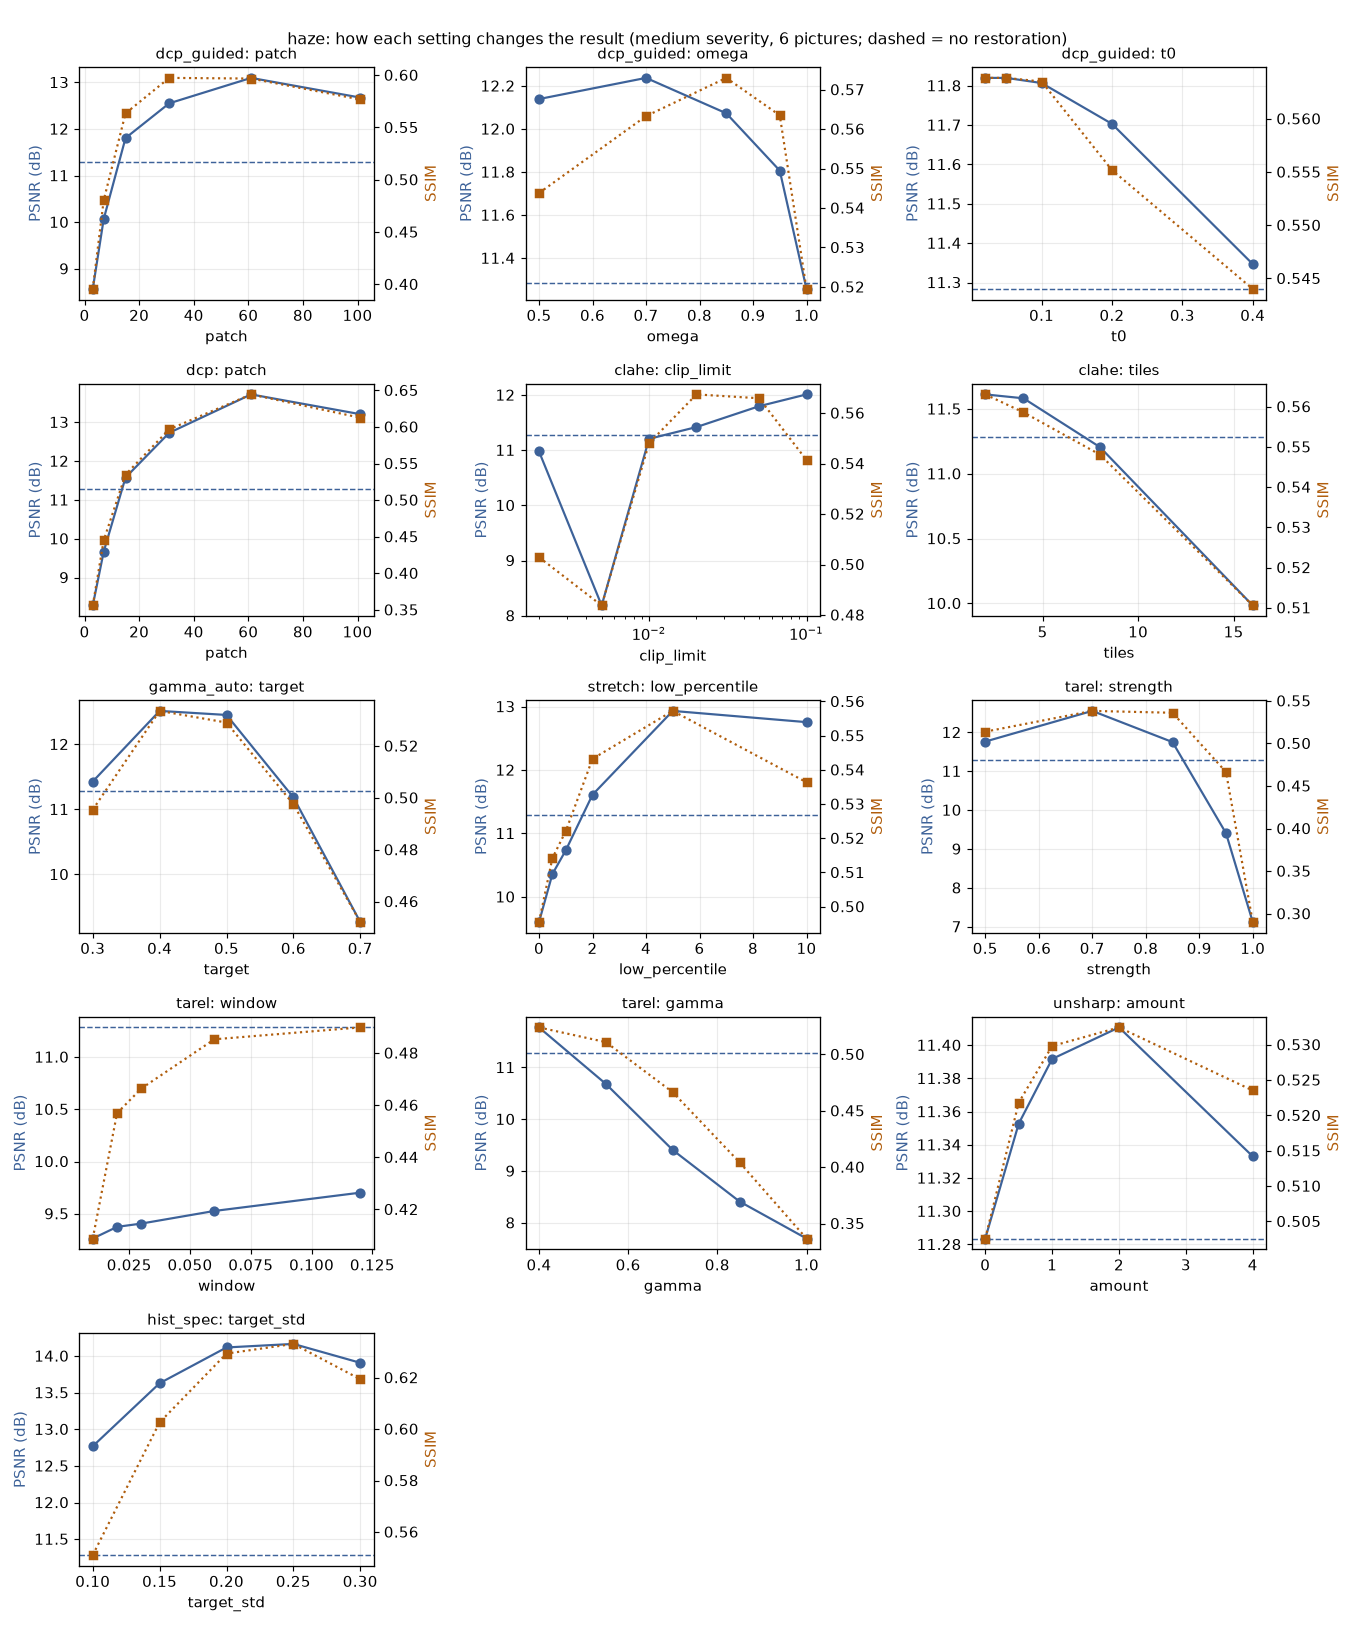
\includegraphics[width=.49\textwidth]{sweeps_haze.png}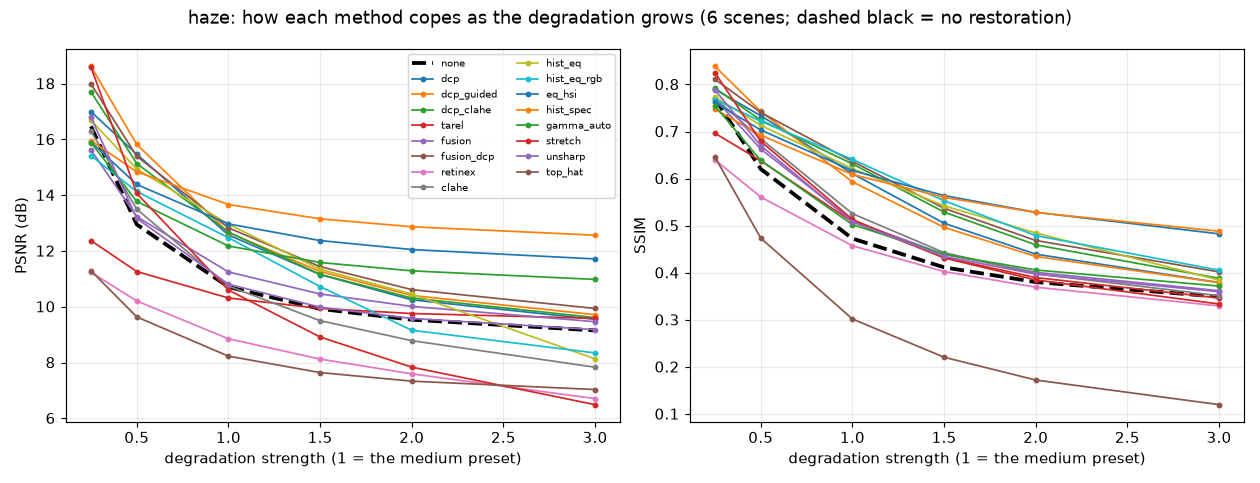
\includegraphics[width=.49\textwidth]{severity_haze.png}\caption{\SYN\ Left: how much a method's own settings matter (haze). Right: score against fog strength (calibrated haze).}\end{figure}
\end{document}
